\documentclass[11pt, openany]{book}
\usepackage{amsmath,amsthm,stmaryrd}
\usepackage{amsfonts}
\usepackage{amssymb}
\usepackage{mathrsfs}
\usepackage[dvips]{graphicx}
\usepackage{color}
\usepackage{pdfpages}


\definecolor{bluedistri}{RGB}{59, 160, 242}
\definecolor{orangedistri}{RGB}{250, 112, 56}
\usepackage{tikz}
\usepackage{pstricks}
\usepackage{pifont}
\newcommand{\cmark}{\ding{51}}
\newcommand{\xmark}{\ding{55}}
\usetikzlibrary{arrows,decorations.pathmorphing,backgrounds,positioning,fit,petri,babel}
\usepackage[ruled,vlined,lined,linesnumbered,algochapter,spanish]{algorithm2e}
\usepackage[T1]{fontenc}
\usepackage{multicol}
%-----------------funcion restricci�n---------------% 
\newcommand{\restr}[1]{\raisebox{-.5ex}{$|$}_{#1}}
\newcommand{\restrd}[2]{{#1}\raisebox{-.5ex}{$|$}_{#2}}
%---------------------------------------------------%
\usepackage[scr=boondoxo,scrscaled=1.05]{mathalfa}
\usepackage[latin1]{inputenc}
\usepackage[spanish,activeacute]{babel}
\usepackage[spanish]{layout}
\usepackage{enumerate}
\usepackage{multirow,hhline}
\usepackage[hidelinks]{hyperref} 
\usepackage{array}
\usepackage[margin=2.5cm]{geometry}
\usepackage{textcomp}
\usepackage{booktabs}



%\renewcommand{\baselinestretch}{1.1}

%%%%%%%%%%%%%%%% Para margenes %%%%%%%%%%%
\hfuzz=20pt
\vfuzz=20pt
\hbadness=2000
\vbadness=\maxdimen
%-----------------------------------------%

%-------------------%DEF DE FUNCION COMPUESTA------------------%
\newcommand{\compcent}[1]{\vcenter{\hbox{$#1\circ$}}}
\newcommand{\comp}{\mathbin{\mathchoice
  {\compcent\scriptstyle}{\compcent\scriptstyle}
  {\compcent\scriptscriptstyle}{\compcent\scriptscriptstyle}}}
%-------------------%DEF DE FUNCION COMPUESTA%-----------------% 

%------------------------------nuevos comandos------------------%
\newcommand{\N}{{\ensuremath{\mathbb{N}}}}
\newcommand{\Z}{{\ensuremath{\mathbb{Z}}}}
\newcommand{\Q}{{\ensuremath{\mathbb{Q}}}}
\newcommand{\R}{{\ensuremath{\mathbb{R}}}}
\newcommand{\C}{{\ensuremath{\mathbb{C}}}}
\newcommand{\K}{{\ensuremath{\mathbb{K}}}}
\newcommand{\J}{{\ensuremath{\mathbb{J}}}}
\newcommand{\s}{{\ensuremath{\mathbb{S}}}}

\newcommand{\mca}{{\ensuremath{\mathcal{A}}}}
\newcommand{\mcb}{{\ensuremath{\mathcal{B}}}}
\newcommand{\mcc}{{\ensuremath{\mathcal{C}}}}
\newcommand{\mcs}{{\ensuremath{\mathcal{S}}}}
\newcommand{\mct}{{\ensuremath{\mathcal{T}}}}
\newcommand{\mcu}{{\ensuremath{\mathcal{U}}}}
\newcommand{\mcp}{{\ensuremath{\mathcal{P}}}}
\newcommand{\mcm}{{\ensuremath{\mathcal{M}}}}
\newcommand{\mcn}{{\ensuremath{\mathcal{N}}}}
\newcommand{\mcj}{{\ensuremath{\mathcal{J}}}}
\newcommand{\mcf}{{\ensuremath{\mathcal{F}}}}
\newcommand{\mcd}{{\ensuremath{\mathcal{D}}}}
\newcommand{\mcx}{{\ensuremath{\mathcal{X}}}}
\newcommand{\mce}{{\ensuremath{\mathcal{E}}}}

\newcommand{\scra}{{\ensuremath{\mathscr{A}}}}
\newcommand{\scrt}{{\ensuremath{\mathscr{T}}}}
\newcommand{\scru}{{\ensuremath{\mathscr{U}}}}
\newcommand{\scrp}{{\ensuremath{\mathscr{P}}}}
\newcommand{\scrv}{{\ensuremath{\mathscr{V}}}}
\newcommand{\scro}{{\ensuremath{\mathscr{O}}}}
\newcommand{\scrb}{{\ensuremath{\mathscr{B}}}}
\newcommand{\scrc}{{\ensuremath{\mathscr{C}}}}
\newcommand{\scrf}{{\ensuremath{\mathscr{F}}}}
\newcommand{\scrs}{{\ensuremath{\mathscr{S}}}}
\newcommand{\scri}{{\ensuremath{\mathscr{I}}}}
\newcommand{\scrj}{{\ensuremath{\mathscr{J}}}}
\newcommand{\scrl}{{\ensuremath{\mathscr{L}}}}
\newcommand{\scrm}{{\ensuremath{\mathscr{M}}}}
\newcommand{\scrn}{{\ensuremath{\mathscr{N}}}}
\newcommand{\scrk}{{\ensuremath{\mathscr{K}}}}
\newcommand{\scre}{{\ensuremath{\mathscr{E}}}}
\newcommand{\scrq}{{\ensuremath{\mathscr{Q}}}}

% Funci\'on salto del gradiente 
\newcommand{\lbt}{\llbracket}
\newcommand{\rbt}{\rrbracket}

% producto interior
\newcommand{\lca}{\langle}
\newcommand{\rca}{\rangle}

\theoremstyle{plain}
  \newtheorem{proposicion}{Proposici\'on}[section]
  \newtheorem{teorema}[proposicion]{Teorema}
  \newtheorem{corolario}[proposicion]{Corolario}
  \newtheorem{lema}[proposicion]{Lema}
  

\theoremstyle{definition}
  \newtheorem{definicion}[proposicion]{Definici\'on}
  \newtheorem{ejemplo}[proposicion]{Ejemplo}
  \newtheorem{ejemplos}[proposicion]{Ejemplos}
  \newtheorem{ejercicio}{Ejercicio}[chapter]
  \newtheorem{ejercicios}{Ejercicios}[chapter]
  \newtheorem{observacion}{Observaci\'on}[chapter]
  \newtheorem*{notacion}{Notaci\'on}
  

\theoremstyle{remark}
\newtheorem*{nota}{Nota}
\newtheorem{consecuencia}{Consecuencia}%[chapter]

\DeclareMathOperator{\inte}{int}
\DeclareMathOperator{\vol}{vol}
\DeclareMathOperator{\supp}{supp}
\DeclareMathOperator{\ips}{\langle \cdot, \cdot\rangle}
\DeclareMathOperator{\norm}{\|\cdot\|}
\DeclareMathOperator{\re}{Re}
\DeclareMathOperator{\id}{id}
\DeclareMathOperator{\im}{Im}
\def\card{\mathop{\rm card}}
\def\diam{\mathop{\rm diam}}
\def\dist{\mathop{\rm dist}}
\def\Lim{\mathop{\rm lim}}
\def\Inf{\mathop{\rm inf}}
\def\Max{\mathop{\rm max}}
\def\Min{\mathop{\rm min}}
\def\Liminf{\mathop{\rm lim\,inf}}
\def\Limsup{\mathop{\rm lim\,sup}}

\newcommand{\cl}{\overline}

\DeclareRobustCommand{\rchi}{{\mathpalette\irchi\relax}}
\newcommand{\irchi}[2]{\raisebox{\depth}{$#1\chi$}} % inner command, used by \rchi
 % si no queremos que a�ada la palabra "Capitulo"
%\addcontentsline{toc}{chapter}{Agradecimientos} % si queremos que aparezca en el �ndice
%\markboth{AGRADECIMIENTOS}{Agradecimiento} % encabezado 
%\addcontentsline{toc}{section}{Resumen} % si queremos que aparezca en el �ndice
%\markboth{RESUMEN}{Resumen} % encabezado
%\usepackage{nopageno}
%\usepackage{fancyhdr}
%\pagestyle{fancy}
%\pagestyle{empty}
\setlength{\headheight}{6mm}
\setlength{\parskip}{11pt}
\setlength{\parindent}{0cm}

\begin{document}
%\fancyhead{}
%\fancyhead[RE]{ \nouppercase \leftmark}
%\fancyhead[LO]{ \nouppercase \rightmark}
%\fancyhead[LE,RO]{\thepage}
%\fancyfoot{}
%\renewcommand{\headrulewidth}{0.6pt}
\bibliographystyle{plain} 

%\renewcommand{\baselinestretch}{1.35}

\makeatletter
\def\@roman#1{\romannumeral #1}
\makeatother


\thispagestyle{empty}
\vspace*{0.5cm}
\begin{center}
	{\Large\scshape Distrifull\\[5pt] }
\end{center}


\vspace*{1cm}
\begin{center}
%	{\large\scshape Avance de proyecto de grado}
\end{center}

\vspace*{1cm}
\begin{center}
	{\Large\scshape Manual de usuario de la p\'agina web}
\end{center}

\vspace*{2cm}
\begin{center}
	{\large\scshape Versi\'on de prueba \\ [3.pt]  }
\end{center}

\vspace*{2cm}
\begin{center}
	{Complejo Ruta N: Calle 67 No 52-20 Piso 1 Oficina 1079, Medell\'in, Colombia. }\\
	\vspace*{.5mm}
	{ 		Recepci\'on de correspondencia: Carrera 80A No 34-36. Tel\'efono 304 638 5898. }\\
	\vspace*{.5mm}
	{ 		Correo electr\'onico: info@asresearch.co
		NIT: 901133054-7}\\
	\vspace{1cm}
	{Medell\'in}\\
\end{center}

\hfill
\begin{center}
	2\ 0\ 2\ 2
\end{center}

%
\includepdf[pages=-]{imagenes/DistrifullLogo}
\pagenumbering{roman}
\frontmatter
\tableofcontents
\listoffigures
%\listoftables
\thispagestyle{empty}
\vspace*{0.5cm}
\begin{flushleft}
	{\Large\scshape \copyright Eureka infinity 2022\\[5pt] }
\end{flushleft}

\vspace*{1cm}
\begin{flushleft}
	%	{\large\scshape Avance de proyecto de grado}
\end{flushleft}

\vspace*{1cm}
\begin{flushleft}
	{\Large\scshape }
\end{flushleft}

\vspace*{2cm}
\begin{flushleft}
	{\large\scshape     }
\end{flushleft}

\vspace*{2cm}
\begin{flushleft}
	{Eureka infinity es mi proyecto personal, su finalidad es publicar todo lo relacionado con la matem\'atica que yo vaya produciendo relacionado con mi entorno,	ya se han cursos, avances de proyectos personales, hasta hoy d\'ia tengo poca experiencia profesional, pero con el tiempo, la disciplina y la constancia en el estudio, estar\'e creciendo gracias a la comunidad.
	 }
\end{flushleft}








\chapter{Introducci\'on}
Este manual de usuario tiene tiene como finalidad dar a conocer  de manera detallada y sencilla la estructura de la web de Distrifull s.a.s, para que los usuarios asociados a la empresa o externos puedan aprovechar al m\'aximo la p\'agina web.

El aplicativo de Distrifull, es una aplicaci\'on que facilita el monitoreo de los tanques de almacenamientos de aceites industriales, proporcionando informaci\'on en tiempo real sobre la capacidad de almacenamiento de los tanques y el costo general del producto.


%\include{AGRADECIMIENTOS}

\pagestyle{plain}
\mainmatter
\part{Mi pc}

La inspiraci\'on no se puede provocar pero se puede estimular realizando tareas simples, antes de cometer otras mas complejas en cualquier caso es un fen\'omeno instintivamente humano y distinto para cada persona.
\chapter{Instalando programas en mi pc}
\section{Terminal}
Para instalar node ejecuto el comando 
\begin{verbatim}
	sudo apt-get install nodejs
\end{verbatim}
Este node es el ultimo estable que se encuentra en los repositorios de Ubuntu, pero descargar la ultima versi\'on ejecutando los siguientes comandos:

\begin{verbatim}
	javier@javier-Lenovo-G40-80:~$ curl -o- https://raw.githubusercontent.com/nvm-sh/nvm/v0.35.3/install.sh | bash
	
	
	javier@javier-Lenovo-G40-80:~$ source ~/.bashrc
	
	javier@javier-Lenovo-G40-80:~$ nvm list-remote
	
	javier@javier-Lenovo-G40-80:~$ nvm install v16.15.0
	
	javier@javier-Lenovo-G40-80:~$ sudo apt-get install npm
	
	
\end{verbatim}

La versi\'on es la necesaria. esa la encontramos en la pagina de nodejs.

Figma: 
\begin{verbatim}
	javier@javier-Lenovo-G40-80:~$ sudo snap install figma-linux
\end{verbatim}

git: 
\begin{verbatim}
	sudo add-apt-repository ppa:git-core/ppa 
	
	sudo apt update 
	
	sudo apt install git
\end{verbatim}
\begin{verbatim}
	javier@javier-Lenovo-G40-80:~$ sudo apt-get update
	Obj:1 http://co.archive.ubuntu.com/ubuntu jammy InRelease
	Obj:2 http://co.archive.ubuntu.com/ubuntu jammy-updates InRelease
	Obj:3 http://security.ubuntu.com/ubuntu jammy-security InRelease
	Obj:4 http://co.archive.ubuntu.com/ubuntu jammy-backports InRelease
	Leyendo lista de paquetes... Hecho
	javier@javier-Lenovo-G40-80:~$ python3
	
	javier@javier-Lenovo-G40-80:~$ sudo apt-get update
	Obj:1 http://co.archive.ubuntu.com/ubuntu jammy InRelease
	Des:2 http://security.ubuntu.com/ubuntu jammy-security InRelease [110 kB]
	Des:3 http://co.archive.ubuntu.com/ubuntu jammy-updates InRelease [109 kB]
	Obj:4 http://co.archive.ubuntu.com/ubuntu jammy-backports InRelease	
\end{verbatim}

Intalando MySQl 

\begin{verbatim}
	https://dev.to/gsudarshan/how-to-install-mysql-and-workbench-on-ubuntu-20-04-localhost-5828 
	
	https://dev.mysql.com/downloads/file/?id=509020 
	
	https://ubuntu.com/server/docs/databases-mysql
\end{verbatim}


\section{Programas instalados desde software Ubuntu}
Texstudio, vscode, Mysql Workbench Community

\part{Python}

Ejecutar Jupyter dentro del entorno virtual, 

\url{https://es.acervolima.com/uso-de-jupyter-notebook-en-un-entorno-virtual/}

Una vez creado el entorno virtual ejecutamos 

abrimos el Jupyter Notebook y procedemos a cambiar el kernel en la opci\'on venv que es como se llamo nuestro kernel, de esta manera podemos acceder a todos los paquetes instalados en nuestro entorno virtual. Para desactivarlo procedemos a ejecutar el siguiente comando: 
\begin{verbatim}
	jupyter-kernelspec uninstall venv
\end{verbatim}
Esto fue consultado en \cite{JupyterEnviroments}.
En si solo es cambiar la direcci\'on del kernel.

Pendiente hacer esto mismo en vscode

\chapter{Numpy}

\section{Dimensiones en matrices}

\subsection{0-D Arrays}
0-D arrays, or scalars, are the elements in a array. Each value in an array is a 0-D array.

\begin{verbatim}
	import numpy as np
	
	arr = np.array(42)
	
	print(arr) 
	
	ouput()
			42
\end{verbatim}


\subsection{1-D Arrays}
An array that has 0-D arrays as its elements is called uni-dimensional or 1-D array.

\begin{verbatim}
Example

Create a 1-D array containing the values 1,2,3,4,5:
import numpy as np

arr = np.array([1, 2, 3, 4, 5])

print(arr) 
print(type(arr)) 
output()
   [1 2 3 4 5]
   <class 'numpy.ndarray'>
\end{verbatim}
No confundir con una lista de Python son totalmente diferentes.


\subsection{2-D Arrays}
An array that has 1-D arrays as its elements is called a 2-D array.

These are often used to represent matrix or 2nd order tensors.

NumPy has a whole sub module dedicated towards matrix operations called numpy.mat

\begin{verbatim}
Example

Create a 2-D array containing two arrays with the values 1,2,3 and 4,5,6:
import numpy as np

arr = np.array([[1, 2, 3], [4, 5, 6]])

print(arr) 
\end{verbatim}




\subsection{3-D Arrays}
An array that has 2-D arrays (matrices) as its elements is called 3-D array.

These are often used to represent a 3rd order tensor.

\begin{verbatim}
Example

Create a 3-D array with two 2-D arrays, both containing two arrays with the values 1,2,3 and 4,5,6:
import numpy as np

arr = np.array([[[1, 2, 3], [4, 5, 6]], [[1, 2, 3], [4, 5, 6]]])

print(arr) 

output()
[ [
  [1 2 3]
  [4 5 6]
  ]
  [
  [1 2 3]
  [4 5 6]
  ]
]
\end{verbatim}


Check Number of Dimensions?

NumPy Arrays provides the ndim attribute that returns an integer that tells us how many dimensions the array have.


\begin{verbatim}
	Example
	
	Check how many dimensions the arrays have:
	import numpy as np
	
	a = np.array(42)
	b = np.array([1, 2, 3, 4, 5])
	c = np.array([[1, 2, 3], [4, 5, 6]])
	d = np.array([[[1, 2, 3], [4, 5, 6]], [[1, 2, 3], [4, 5, 6]]])
	
	print(a.ndim)
	print(b.ndim)
	print(c.ndim)
	print(d.ndim) 
	output()
	0
	1
	2
	3
\end{verbatim}

Higher Dimensional Arrays

An array can have any number of dimensions.

When the array is created, you can define the number of dimensions by using the ndmin argument.

\begin{verbatim}
	Example
	
	Create an array with 5 dimensions and verify that it has 5 dimensions:
	import numpy as np
	
	arr = np.array([1, 2, 3, 4], ndmin=5)
	
	print(arr)
	print('number of dimensions :', arr.ndim) 
	
	output()
	[[[[[1 2 3 4]]]]]
	number of dimensions : 5
\end{verbatim}
In this array the innermost dimension (5th dim) has 4 elements, the 4th dim has 1 element that is the vector, the 3rd dim has 1 element that is the matrix with the vector, the 2nd dim has 1 element that is 3D array and 1st dim has 1 element that is a 4D array.

\section{Numpy data types}

Data Types in Python

By default Python have these data types:

strings - used to represent text data, the text is given under quote marks. e.g. ``ABCD''


integer - used to represent integer numbers. e.g. -1, -2, -3

float - used to represent real numbers. e.g. 1.2, 42.42

boolean - used to represent True or False.

complex - used to represent complex numbers. e.g. 1.0 + 2.0j, 1.5 + 2.5j

Data Types in NumPy

NumPy has some extra data types, and refer to data types with one character, like i for integers, u for unsigned integers etc.

Below is a list of all data types in NumPy and the characters used to represent them.

i - integer\\
b - boolean\\
u - unsigned integer\\
f - float\\
c - complex float\\
m - timedelta\\
M - datetime\\
O - object\\
S - string\\
U - unicode string\\
V - fixed chunk of memory for other type ( void )\\


Shape of an Array

The shape of an array is the number of elements in each dimension.

Get the Shape of an Array

NumPy arrays have an attribute called shape that returns a tuple with each index having the number of corresponding elements.

The shape arrays is return tupla where, first element is 

L aforma de un arreglo 


Estudiando de 
\url{https://www.w3schools.com/python/numpy/numpy_array_join.asp} y python para Data Science

\section{Shape de un arreglo}
Un array o arreglo de numpy tiene un atributo llamado shape que retorna una tupla donde cada indice tiene el numero correspondiente de elementos, ejemplo: 
\begin{verbatim}
	Example
	
	Print the shape of a 2-D array:
	import numpy as np
	
	arr = np.array([[1, 2, 3, 4], [5, 6, 7, 8]])
	
	print(arr.shape) 
	
	output: 
	
	(2,4)
	
	Nos \'indica que tenemos un arreglo de dos elementos de una
	dimensi\'on y cada elemenos de una dimensi\'on tiene cuatro elementos.
	
	import numpy as np
	
	arr = np.array([1, 2, 3, 4], ndmin=5)
	
	print(arr)
	print('shape of array :', arr.shape) 
	import numpy as np
	
	arr = np.array([1, 2, 3, 4], ndmin=5)
	
	print(arr)
	
	print('shape of array :', arr.shape)
	
	[[[[[1 2 3 4]]]]]
	shape of array : (1, 1, 1, 1, 4)
\end{verbatim}

\section{NumPy Array Reshaping}

Reshaping o reformar un array o arreglo significa cambiar la forma de un array, el shape de un arreglo es el n\'umero de elementos en cada dimenci\'on. Al reshaping podemos agregar o eliminar dimensiones o cambiar el n\'umero de elementos en cada dimensi\'on. 

\subsection{Reshape de 1-D a 2-D}

Ejemplo: 

Convirtamos el siguiente array de  1-D con 12 elementos en un arreglo de 2-D, donde la dimensi\'on 2-D tendra 4 elementos y cada elemento de una dimensi\'on tendra 3 elementos.

\begin{verbatim}
	import numpy as np
	
	arr = np.array([1, 2, 3, 4, 5, 6, 7, 8, 9, 10, 11, 12])
	
	newarr = arr.reshape(4, 3)
	
	print(newarr)
	
	output:
	[[ 1  2  3]
	[ 4  5  6]
	[ 7  8  9]
	[10 11 12]]
\end{verbatim}

Ahora convirtamos el arreglo de 1-D en un arreglo en 3-D, es decir: 

\begin{verbatim}
	import numpy as np
	
	arr = np.array([1, 2, 3, 4, 5, 6, 7, 8, 9, 10, 11, 12])
	
	newarr = arr.reshape(2, 3, 2)
	
	print(newarr) 
	output:
	
	import numpy as np
	
	arr = np.array([1, 2, 3, 4, 5, 6, 7, 8, 9, 10, 11, 12])
	
	newarr = arr.reshape(2, 3, 2)
	
	print(newarr)
	
	[[[ 1  2]
	[ 3  4]
	[ 5  6]]
	
	[[ 7  8]
	[ 9 10]
	[11 12]]]
\end{verbatim}

El elemento retornado tiene la misma direcci\'on de memoria el arreglo original, es decir sucede lo siguiente:
\begin{verbatim}
	import numpy as np
	
	arr = np.array([1, 2, 3, 4, 5, 6, 7, 8, 9, 10, 11, 12])
	
	newarr = arr.reshape(4, 3)
	newarr[1][0]=2
	print(newarr)
	print(arr)
	output: 
	[[ 1  2  3]
	[ 2  5  6]
	[ 7  8  9]
	[10 11 12]]
	
	[ 1  2  3  2  5  6  7  8  9 10 11 12]
\end{verbatim}


\section{M\'etodos}




\part{Lenguajes del frontend}

\chapter{Figma}

\chapter{JavaScript}


Funciones de Flecha, 

ES5 //JSON.parse(JSON.stringify(paddockType));

\chapter{Typescript}

\chapter{Next.js}

El objetivo de aprender este lenguaje es darle asistencia a la p\'agina de As-research, junto con el blog. 

Me estare guiando de \url{https://nextjs.org/docs/getting-started}

Foro de discusiones: \url{https://github.com/vercel/next.js/discussions}

Requerimientos del sistema: 

Node.js 12.22.0 or later\\
MacOS, Windows (including WSL), and Linux are supported


C\'omo iniciar un proyecto?

Para construir una aplicaci\'on web completa con React desde cero, hay muchos detalles importantes que tu necesitas considerar: 
\begin{enumerate}
	\item C\'odigo tiene que ser empaquetado usando un empaquetador como webpack y transformarlo utilizando un copilador como Babel.
	\item Debes realizar optimizaciones de producci\'on, como la divisi\'on de c\'odigo.
	\item Es posible que desee renderizar previamente est\'aticamente algunas p\'aginas para mejorar el rendimiento y el SEO. Tambi\'en es posible que desee utilizar la representaci\'on del lado del servidor o la representaci\'on del lado del cliente.
	
	
	\item Es posible que deba escribir alg\'un c\'odigo del lado del servidor para conectar su aplicaci\'on React a su almac\'en de datos.
\end{enumerate}
\begin{verbatim}
npx create-next-app nextjs-blog

Para recorrer el servidor del proyecto es:

npm run dev
\end{verbatim}






\chapter{Una cota superior para el error}
El objetivo principal es encontrar una cota superior para el error $\|u-u_{h}\|_{1}$, que dependa de los datos dados de la ecuaci\'on diferencia cl\'asica  y la soluci\'on $u_{h}$ del problema discreto, para llevar acabo nuestro objetivo nos hemos guiado de Verf\"urth \cite[pp. 1-12]{Rudiger2013} que muestra una cota superior para el problema cl\'asico con condici\'on de frontera tipo mixta, con cierto \'enfasis de Braess \cite[pp. 172-175]{Dietrich2007} particularizando para el problema cl\'asico con condici\'on de frontera tipo Dirichlet. De \cite{Ciarlet1978} hacemos un breve repaso del m\'etodo de los elementos finitos, para lograr una afinidad en la construcci\'on de los espacios de dimensi\'on finita que tienen un rol muy importante en lo que resta de la monograf\'ia. 

\section{M\'etodo de los elementos finitos (FEM)}
En el capitulo anterior los problemas cl\'asicos de la ecuaci\'on de Poisson, se ha podido formular en un sistema matricial, el cual resolveremos sobre espacios de funciones de dimensi\'on finita utilizando el m\'etodo de elementos finitos.

El m\'etodo de los elementos finitos seg\'un Ciarlet \cite[pp. 55-60]{Ciarlet1978}, en su forma m\'as simple es un proceso especifico de construcci\'on de subespacios $S_{h}$, que se denomina espacio de elementos finitos, esta construcci\'on es caracterizada por tres aspectos b\'asicos, que son (FEM 1), (FEM 2) y (FEM 3).

\begin{definicion}
Un $n$-s\'implex es la envoltura convexa de un conjunto $K\subset \R^{n}$ de $(n + 1)$ puntos independientes, definidos como $N_{i}=(N_{i,j})_{j=1}^{n} \in \R^{n}$ con $1\leq i\leq n+1$, son llamados los v\'ertices del $n$-s\'implex. Para cualquier entero $m$ con $ 0\leq m \leq n$, una $m$-cara del $n$-s\'implex $K$,  es un $m$-s\'implex, cuyos $m + 1$ v\'ertices son tambi\'en v\'ertices de $K$. En particular una $(n-1)$-cara es simplemente llamada una cara y $1$-cara es simplemente llamado borde o lado.  Definimos el siguiente arreglo matricial 
\begin{equation}
C\mcn=\begin{pmatrix}
N_{1,1}& N_{1,2} & \ldots & N_{1,n} & 1 \\
N_{2,1}& N_{2,2} & \ldots & N_{2,n} & 1 \\
\vdots &  \vdots & \ldots & \vdots  & 1 \\
N_{n+1,1}& N_{n+11,2} & \ldots & N_{n+1,n} & 1 \\
\end{pmatrix},
\end{equation}
cada fila de $C\mcn$ hasta la columna n, son las coordenadas de los v\'ertices del $n$-s\'implex.

Las coordenadas baricentricas, son funciones $\lambda_{i}(x_{1},x_{2},\ldots,x_{n})$ definidas en cada v\'ertice del $n$-s\'implex tal que 
\begin{equation}
\begin{split}
\lambda_{i}(x_{1},x_{2},\cdots,x_{n})&=\sum_{j=1}^{n} b_{j,i}x_{j} + b_{n+1,1}, \quad \text{ con } 1\leq i\leq n+1,\\
\lambda_{i}(N_{j})&= \delta_{ij}=\begin{cases}
1, \text{ si }i=j\\
0, \text{ si }i\neq j
\end{cases} \text{ con } 1\leq i,j\leq n+1,
\end{split}
\end{equation}
donde $B=(b_{i,j})_{i,j=1}^{n+1}$ es la matriz inversa de $C\mcn$.
\end{definicion}

Consideremos el espacio $\R^{n}$ con su base can\'onica $(e_{i})_{i=1}^{n}$ y definimos el espacio $\mcp_{k}(\R^{n})\colon = \{ p: \R^{n}\to \R \mid\text{ p es un polinomio con } grad(p)\leq k \}$, un $p\in\mcp_{k}(\R^{n})$ tiene la siguiente forma
\begin{equation}\label{FEM1}
\begin{split}
p\colon (x_{1},\cdots,x_{n}) \in \R^{n} &\to p(x_{1},\cdots,x_{n}) = \sum_{|\alpha|\leq k} \rho_{\alpha_{1}\alpha_{2}\cdots\alpha_{n}}x_{1}^{\alpha_{1}}x_{2}^{\alpha_{2}}\cdots x_{n}^{\alpha_{n}} ,
\end{split}
\end{equation}
la dimensi\'on de $\mcp_{k}$ es 
\[ dim\mcp_{k} = \binom{n+k}{k} \]
\begin{ejemplo}\label{FEM2}
Considerando $k=1$ y $n=2$ determinemos $\mcp_{1}(\R^{2})$, el 2-s\'implex con v\'ertices $N_{1}=(0,0), N_{2}=(1,0), N_{3}=(1/2,1)$ y las coordenadas baricentricas.

para determinar la forma de $p\in\mcp_{1}(\R^{2})$, es decir el polinomio $p:\R^{2}\to \R$, los posibles $\rho$ son $\rho = (0,0) , \rho = (1,0)$ y $\rho=(0,1)$, en cada caso $|\alpha|\leq 1$ as\'i 
\begin{equation*}
\begin{split}
p(x_{1},x_{2})&=\sum_{|\rho|\leq 1} {\rho_{1}\rho_{2}}x_{1}^{\rho_{1}} x_{2}^{\rho_{2}},\\
&=\rho_{1}\rho_{0} x^{0}_{1}x^{0}_{2} + \rho_{1}\rho_{1}x_{1}x^{0}_{2} + \rho_{0}\rho_{1}x^{0}_{1}x^{1}_{2},\\
\end{split}
\end{equation*} 
consideremos $\gamma=\rho_{0}\rho_{1}$, $\alpha = \rho_{1}\rho_{0}$ y $\beta=\rho_{0}\rho_{1}$, as\'i 
\[ \mcp_{1}(\R^{n})\colon = \{ \alpha_{i} x_{1} + \beta_{i} x_{2} + \gamma_{i} \mid \gamma_{i},\alpha_{i},\beta_{i}\in \R    \}. \]

El 2-s\'implex :
\begin{figure}[h!]\label{figura1}
	\begin{center}
	\begin{tikzpicture}
	[place/.style={circle,draw=blue!100,fill=blue!20,thick,
		inner sep=0pt,minimum size=1mm},
	place1/.style={circle,draw=black!100,fill=black!100,thick,
		inner sep=0pt,minimum size=1mm},
	place2/.style={circle,draw=red!100,fill=red!70,thick,
		inner sep=0pt, minimum size=1mm},
	place3/.style={circle,draw=red!100,fill=red!20,thick,
		inner sep=0pt, minimum size=0.7mm},scale=1.5]
	\draw[black!50,line width=1pt]


(0,0)node[place]{}--(1,0)node[place1]{} -- (0.5,1)node[place1]{} -- (0,0)node[place1]{} ;
	
	%funcionesbaricentricas 
	\node at (-0.2,-0.2) [] {$\lambda_{1},N_1$};
	\node at (1.2,-0.2) [] {$\lambda_{2},N_{2}$};
	\node at (0.5,1.3) [] {$\lambda_{3},N_3$};
	\end{tikzpicture}
\end{center}
\caption{Representaci\'on de las coordenadas baricentricas y nodos en el 2-s\'implex }
\setlength{\abovecaptionskip}{0pt}
\setlength{\belowcaptionskip}{0pt}
\end{figure}

La matrices $C\mcn$ y $B$ son 
\begin{equation*}
\begin{split}
C\mcn=\begin{pmatrix}
0 & 0 & 1\\
1 & 0 & 1 \\
0.5 & 1 & 1
\end{pmatrix}
\quad \text{ y }\quad B= \begin{pmatrix}
-1 & 1 & 0\\
-0.5 & -0.5 & 1 \\
1 & 0 & 0
\end{pmatrix},
\end{split}
\end{equation*}  
las coordenadas baricentricas son 
\begin{equation*}
\begin{split}
\lambda_{1}(x_{1},x_{2}) &= -x_{1} - 0.5x_{2} +1 ,  \\
\lambda_{2}(x_{1},x_{2}) &= x_{1} - 0.5x_{2} + 0 ,  \\
\lambda_{3}(x_{1},x_{2}) &= 0x_{1} + x_{2} + 0 .  \\
\end{split}
\end{equation*}
Notemos que los coeficientes de cada coordenada baricentrica corresponde a una columna de $B$.
\end{ejemplo}

Para la construci\'on de los espacios $S_{h}$ en la formulaci\'on discreta \eqref{eq3}, en esta monograf\'ia utilizamos 2-s\'implex, particularmente tri\'angulos rect\'angulos is\'osceles.

\begin{enumerate}[{\rm (FEM 1)}]
\item  En esta etapa del proceso, se establece una partici\'on o subdivisi\'on de $\overline{\Omega}$ que llamamos $\mct_{h}$, que tiene un  n\'umero finito de subconjuntos $T$, que se denominan elementos finitos. $\mct_{h}$  se elige de tal manera que satisface las siguientes propiedades:
\begin{enumerate}[{\rm  (1)}]
\item  $\overline{\Omega}= \bigcup_{T\in \mct_{h} } T$.
\item Para cada $T\in \mct_{h}$, $T$ es cerrado y $int(T)\neq\emptyset$.
\item Para cada $T_{1},T_{2}\in \mct_{h}$ distintos, se tiene que $int(K_{1})\cap int(T_{2})=\emptyset$.
\item Para cada $T\in \mct_{h}$, $\partial T$ es Lipschitz-continua.
\item Para cada $T_{1},T_{2}\in \mct_{h}$ distintos, son adyacentes si  $T_{1}\cap T_{2}$ es una cara, que es la misma cara para ambos o adyacentes a la frontera $\partial\Omega$ cuando al menos una cara hace parte de $\partial\Omega$.
\end{enumerate}
\end{enumerate} 
Las siguientes figuras son ejemplos de una subdivisi\'on en un conjunto $\Omega$.
\begin{figure}[h]\label{figura2}
\begin{center}
		\begin{tikzpicture}
		[place/.style={circle,draw=blue!100,fill=blue!20,thick,
			inner sep=0pt,minimum size=1mm},
		place1/.style={circle,draw=black!100,fill=black!100,thick,
			inner sep=0pt,minimum size=1mm},
		place2/.style={circle,draw=red!100,fill=red!70,thick,
			inner sep=0pt, minimum size=1mm},
		place3/.style={circle,draw=red!100,fill=red!20,thick,
			inner sep=0pt, minimum size=0.7mm},scale=1.5]
		%  Omega con los triangulos 
%		\draw[<->] (0,-1.5) -- (0,1.5);
%		\node at (0.2,1.5){$y$};
%		\draw[<->] (-1.5,0) -- (1.5,0);
%		\node at (1.5,0.2) {$x$};
%		\draw[black!100,line width = 1pt] 
%		(-1,-1) -- (1,-1) -- (1,1) -- (-1,1)--(-1,-1);
		%    nodos de los triangulos 
%		\node[place] at (0,0) {$\Omega$};
		% tercer Omega con fronteras
		%---------------------primera linea ------------
		%\draw [->,line width=2pt,red] (3,3) -- (4.5,3);    
%		\node at (-1,-1.2) {$a$};
%		\node at (1,-1.2) {$b$};
%		\node at (-1,1.2) {$c$};
%		\node at (1,1.2) {$d$};
		%---------------------segundo cuadrado---------
		\draw[black!50,line width=1pt] (2,-1)node[place1]{}--(3,-1)node[place1]{} -- (4,-1)node[place1]{} -- (4,0)node[place1]{} -- (3,-1)node[place1]{}--(3,0)node[place1]{}--(2,-1)node[place1]{} --(2,0)node[place1]{}--(4,0)node[place1]{}--(4,1)node[place1]{}--(3,0)node[place1]{}--(3,1)node[place1]{}--(2,0)node[place1]{}--(2,1)node[place1]{}--(4,1) ;
		
		%----h------
		\draw[black!50, line width=1pt]
		(2,1.2)node{|}  -- (3,1.2)node{|};
		\node at (2.5,1.4) {$h$};
		%-----------
		
		
		\draw[black!30,line width=1pt] (5,-1)node[place1]{}--(6,-1)node[place1]{} -- (7,-1)node[place2]{} -- (7,0)node[place1]{} -- (6,-1)--(6,0)node[place1]{}--(5,-1) --(5,0)node[place1]{}--(7,0)--(7,1)node[place1]{}--(6,0)--(6,1)node[place1]{}--(5,0)--(5,1)node[place1]{}--(7,1) ;
		\draw[black!100,line width=1pt] (7,-1)node[place2]{}-- (6.5,-0.5)node[place2]{} ;
		\node at (3,-1.5) [fill=red!10,decorate] {{\bf $\mct_{h}$}};
		\node at (6,-1.5) [fill=red!10,decorate] {{\bf $\mct$}};
		%nodos de los triangulos 
		\node at (2.3,-0.3) [place] {$T_{1}$};
		\node at (2.7,-0.7) [place] {$T_{2}$};
		\node at (3.3,-0.3) [place] {$T_{3}$};
		\node at (3.7,-0.7) [place] {$T_{4}$};
		
		\node at (2.3,0.7) [place] {$T_{5}$};
		\node at (2.7,0.3) [place] {$T_{6}$};
		\node at (3.3,0.7) [place] {$T_{7}$};
		\node at (3.7,0.3) [place] {$T_{8}$};
		
		\node at (5.3,-0.3) [place] {$T_{1}$};
		\node at (5.7,-0.7) [place] {$T_{2}$};
		\node at (6.3,-0.3) [place] {$T_{3}$};
		\node at (6.5,-0.8) [place3,transform shape,scale=0.5] {$T_{4}$};
		\node at (6.8,-0.5) [place3,transform shape,scale=0.5] {$T_{5}$};
		
		\node at (5.3,0.7) [place] {$T_{6}$};
		\node at (5.7,0.3) [place] {$T_{7}$};
		\node at (6.3,0.7) [place] {$T_{8}$};
		\node at (6.7,0.3) [place] {$T_{9}$};
		\end{tikzpicture}
\end{center}
\caption{Representaci\'on de dominios, $\mct_{h}$ que satisface (FEM 1) y $\mct$ que no satisface (FEM 1) }
\setlength{\abovecaptionskip}{0pt}
\setlength{\belowcaptionskip}{0pt}
\end{figure}

Notemos que la figura \ref{figura2} la triangulaci\'on en la parte derecha no se cumple la propiedad 5 de (FEM 1), mientras que la tri\'angulaci\'on de la parte izquierda, si cumple todas las propiedades de (FEM 1).

De Verf\"uth \cite{Rudiger2013} asociamos la siguiente notaci\'on. Para  la subdivisi\'on o partici\'on $\mct_{h}$ asociamos el conjunto $\mcn$  y $\mce$ de todos los v\'ertices  y lados, respectivamente de todos los elementos en $\mct_{h}$. Un sub\'indice $T,\Omega,\Gamma, \Gamma_{D}$, o $\Gamma_{N}$ a $\mcn$ o $\mce$ indica que solo se toman los v\'ertices o lados que est\'an contenidos en el conjunto del sub\'indice, respectivamente.  Similarmente $\mcn_{e}$ denota el conjunto de los v\'ertices de un lado $E$. La uni\'on de todos los lados en $\mce$ es denotada por $\mce_{\Sigma}$ y es llamado el esqueleto de $\mct_{h}$. 

Con cada elemento $T$, cada lado $e$, y cada v\'ertice $N$ asociamos los siguientes conjuntos. 
\begin{equation*}
\begin{aligned}
\omega_{e} &= \bigcup\{ T^{\prime} \mid e\in \mce_{T^{\prime}} \} \\
\omega_{\text{\tiny $N$}} &= \bigcup \{ T^{\prime} \mid N\in\mcn_{T^{\prime}} \}
\end{aligned}
\qquad
\begin{aligned}
\widetilde{\omega}_{\textit{\tiny T}} &= \bigcup\{ T^{\prime} \mid \mcn_{e}\cap \mcn_{T^{\prime}} \}, \\
\qquad \widetilde{\omega}_{e}&= \bigcup \{ T^{\prime} \mid \mcn_{e}\cap \mcn_{T^{\prime}}\neq \emptyset \}.
\end{aligned}
\end{equation*}
\begin{figure}[h]\label{figura3}
\begin{center}
	\begin{tikzpicture}
	[place/.style={circle,draw=black!60,fill=black!20,thick,
		inner sep=0pt,minimum size=0.2mm},
	place1/.style={circle,draw=black!100,fill=black!100,thick,
		inner sep=0pt,minimum size=1mm},
	place2/.style={circle,draw=red!100,fill=red!70,thick,
		inner sep=0pt, minimum size=1mm},
	place3/.style={circle,draw=red!100,fill=red!20,thick,
		inner sep=0pt, minimum size=0.7mm},scale=1.5]
%primer tri\'angulo
\draw[black!50,line width=1pt]
(-1,0)node[place]{}  -- (-0.5,0.5)node[place1]{} -- (0,0)node[place1]{} --  (-0.5,-0.5)node[place1]{} -- (-1,0)node[place1]{};
%\node at (-0.5,-0.8) [] {$w_{e}$} ;
\node at (-0.5,0.1) [] {$e$} ;
\draw[black!90,line width=1.5pt]
(-1,0)node[place1]{} -- (0,0)node[place1]{};

%segunda figura 
\draw[black!50,line width=1pt]
(1,0)node[place]{}  -- (1.5,0.5)node[place1]{} -- (2,0)node[place1]{} --  (1.5,-0.5)node[place1]{} -- (1,0)node[place1]{} -- (0.5,0.5)node[place1]{} -- (0.5,-0.5)node[place1]{} -- (1,0)node[place1]{} ;
\draw[black!90,line width=1.5pt]
(1,0)node[place1]{} -- (2,0)node[place1]{};
\draw[black!50,line width=1.5pt]
(0.5,-0.5)node[place1]{} -- (1.5,-0.5)node[place1]{} -- (2.5,-0.5)node[place1]{} -- (2,0)node[place1]{} -- (2.5,0.5)node[place1]{} -- (0.5,0.5)node[place1]{};
\draw[black!50,line width=1.5pt]
(2.5,0.5)node[place1]{} -- (2.5,-0.5)node[place1]{};
%\node at (1.5,-0.8) [] {$\widetilde{\omega}_{e}$};
\node at (1.5,0.1) [] {$e$};
% tercera figura
\draw[black!50,line width=1pt]
(3.5,0)node[place]{}  -- (4,0.5)node[place1]{} -- (4.5,0)node[place1]{} --  (4,-0.5)node[place1]{} -- (3.5,0)node[place1]{} -- (3,0.5)node[place1]{} -- (3,-0.5)node[place1]{} -- (3.5,0)node[place1]{} ;
\draw[black!50,line width=1.5pt]
(3.5,0)node[place1]{} -- (4.5,0)node[place1]{};
\draw[black!50,line width=1.5pt]
(3,-0.5)node[place1]{} -- (4,-0.5)node[place1]{} -- (5,-0.5)node[place1]{} -- (4.5,0)node[place1]{} -- (5,0.5)node[place1]{} -- (3,0.5)node[place1]{};
\draw[black!50,line width=1.5pt]
(5,-0.5)node[place1]{} -- (5,0.5)node[place1]{} -- (4.5,1)node[place1]{} -- (4,0.5)node[place1]{} -- (3.5,1)node[place1]{} -- (3,0.5)node[place1]{};
\draw[black!50,line width=1.5pt]
(3.5,1)node[place1]{} -- (4.5,1)node[place1]{};
%\node at (4,-0.8) [] {$\widetilde{\omega}_{\textit{\tiny T}}$};
\node at (4,0.25) [] {$T$};
\draw[black!50,line width=1.5pt]
(6,-0.5)node[place1]{} -- (6.5,0)node[place1]{} -- (7,-0.5)node[place1]{} -- (7.5,0)node[place1]{} -- (7,0.5)node[place1]{} -- (6.5,0)node[place1]{} -- (6,0.5)node[place1]{} -- (5.5,0)node[place1]{} -- (6,-0.5)node[place1]{};
\draw[black!50,line width=1.5pt]
(6,-0.5)node[place1]{} -- (7,-0.5)node[place1]{};
\draw[black!50,line width=1.5pt]
(5.5,0)node[place1]{} -- (6.5,0)node[place1]{} -- (7.5,0)node[place1]{};
\draw[black!50,line width=1.5pt]
(6,0.5)node[place1]{} -- (7,0.5)node[place1]{};
\node at (6.5,0) [place] {$\textit{\tiny N}$};
%\node at (6.5,-0.7) {$\sigma_{N}$};
\end{tikzpicture}
\end{center}
\caption{Representaci\'on de $\omega_{e}$, $\widetilde{\omega}_{e}$, $\widetilde{\omega}_{\textit{\tiny T}}$, $\omega_{\text{\tiny $N$}}$ se corresponde de izquierda a derecha con las gr\'aficas}
\setlength{\abovecaptionskip}{0pt}
\setlength{\belowcaptionskip}{0pt}
\end{figure}

En la subdivisi\'on $\mct_{h}$ se define un espacio de elementos finitos $S_{h}$, que se especifica en el proceso, por ejemplo para los problemas discretos, el espacio de elementos finitos, cuando tenemos la condici\'on de frontera tipo Dirichlet no homog\'eneo y Neumann es
\begin{equation}
S_{h}^{1}= \{ v\in C^{1}(\overline{\Omega})\colon  v\restr{T}\in\mcp_{1}, \quad \forall T\in \mct_{h} \},
\end{equation}
para el caso tipo  Dirichlet homog\'eneo, y mixtas tenemos 
\[ S_{0h}^{1}= \{ v\in C^{1}(\overline{\Omega})\colon  v\restr{T}\in \mcp_{1}, \quad \forall T\in \mct_{h}, v\restr{\Gamma_{D}}\equiv 0  \}. \]
\begin{enumerate}[{\rm (FEM 2)}]
\item El segundo aspecto del m\'etodo de los elementos finitos es la construcci\'on de los espacios de elementos finitos como espacios de funciones de polinomios, este hecho tiene una gran importancia ya que al realizar la implementaci\'on computacional los c\'alculos de los coeficientes del sistema \eqref{eq8} son mas simples. 
\end{enumerate}

En Ciarlet \cite[p. 78]{Ciarlet1978} nos presenta una definici\'on m\'as general de elemento finito que se enfoca en el espacio de funciones y las funciones base locales del elemento finito, ya que hasta ahora en (FEM 1) el elemento finito solo se ve como al objeto geom\'etrico elegido para hacer la subdivisi\'on o partici\'on de $\Omega$. 
\begin{definicion}
Un elemento finito en $\R^{n}$ es una tripleta $(T,P,\Sigma)$  donde : 
\begin{enumerate}[{\rm (i)}]
	\item $T$ es un subconjunto cerrado de $\R^{n}$ con $int(T)\neq \emptyset$ y frontera Lipschitz-continua. 
	\item $P$ es un espacio de funciones real-valuadas definidas sobre el conjunto $T$. 
	\item $\Sigma$ es un conjunto finito de funciones linealmente independiente $\phi_{i}$, con $1\leq i \leq n+1$, sobre $P$. 
\end{enumerate}
\end{definicion}
\begin{ejemplo}
	Considerando  $T$ como el 2-s\'implex en el ejemplo \eqref{FEM2}, se tiene que $p=\mcp_{1}(T)$ y $\Sigma$ esta conformado por las funciones de las coordenadas baricentricas, es decir $\Sigma =\{ \lambda_{1},\lambda_{2},\lambda_{3} \}$, as\'i el elemento finito es la tripleta $(T,P,\Sigma)$ 
\end{ejemplo}

\begin{definicion}
Dos elementos finitos $(T,P,\Sigma)$ y $(\widehat{T},\widehat{P},\widehat{\Sigma})$, son equivalentes-af\'in, si existe una funci\'on invertible $F\colon \widehat{T} \to T$, tal que las siguientes relaciones se cumplen 
\begin{enumerate}[{\rm (i)}]
	\item $T=F(\widehat{T})$,
	\item $P = \{ p:T\to \R  \mid p\equiv\widehat{p}\comp F^{-1},\quad  \widehat{p}\in \widehat{P} \},$
	\item $N_{i}=F(\widehat{N}_{i})$ para $1 \leq i\leq n+1,$
	\item $\Sigma = \{ \phi_{i}(F(\widehat{N}_{i})) \mid 1\leq i\leq n+1 \}. $
\end{enumerate}
\end{definicion}
Una familia de elementos finitos $\mct_{h}$ se denomina familia af\'in, si todos sus elementos finitos son af\'in-equivalentes a un solo elemento finito no necesariamente contenido en la familia de elementos finitos $\mct_{h}$, que se llama el elemento finito de referencia de la familia $\mct_{h}$.

\begin{ejemplo}
Dada una familia de elementos finitos simpliciales en $\R^{n}$, es muy com\'un elegir como elemento de referencia a la unidad $n$-s\'implex con v\'ertices 
\begin{equation*}
\begin{split}
\widehat{N}_{1}& = (1,0,\ldots,0),\\
\widehat{N}_{2}& = (0,1,\ldots,0),\\
& \vdots \\
\widehat{N}_{n}& = (0,0,\ldots,1),\\
\widehat{N}_{n+1}& = (0,0,\ldots,0),
\end{split}
\end{equation*}
con coordenadas baricentricas 
\[ \lambda_{i} = x_{i},\quad 1\leq i\leq n \text{ y } \lambda_{n+1}=1-\sum_{i=1}^{n}x_{i}, \]

en caso de una familia af\'in rectangular de elementos finitos, usualmente se elige el elemento de referencia como el hipercubo unitario $[0,1]^{n}$ o el hipercubo $[-1,1]^{n}$.
\end{ejemplo}

El concepto de familia af\'in es importante ya que en la practica, la mayor parte del trabajo involucrado en los c\'alculos de los coeficientes del sistema \eqref{eq8} se realiza en elementos finitos de referencia y no en los elementos finitos de la familia. 

\begin{enumerate}[{\rm (FEM 3)}]
	\item El tercer aspecto del m\'etodo de elementos finitos es que existe al menos una base can\'onica en el espacio $S_{h}$, cuyas funciones base correspondientes tienen soporte lo mas peque\~no. 
\end{enumerate}

Hasta ahora de $(FEM 1)$ y $(FEM 2)$ tenemos localmente para cada $T\in\mct_{h}$,  el espacio de funciones $P$ y el conjunto de funciones bases local $\Sigma$. Ahora definamos 
\[ \mcn_{h} \colon = \bigcup_{T\in \mct_{h}} \mcn_{T},  \] 
son los nodos o v\'ertices de $\mct_{h}$. 
El conjunto del n\'umero de grados de libertad del espacio de elementos finitos es el conjunto 
\[\Sigma_{h}=\{ \varphi(N)\mid N\in \mcn_{h} \}, \]
donde $\varphi(N)$ es la funci\'on base global correspondiente al nodo $N$, el conjunto $\Sigma_{h}$ se llama el conjunto de grados de libertad del espacio de elementos finitos.
\begin{figure}[h]\label{figura4}
\begin{center}
	\begin{tikzpicture}
	[place/.style={circle,draw=black!70,fill=black!40,thick,
		inner sep=0pt,minimum size=0.5mm},
	place1/.style={circle,draw=black!100,fill=black!100,thick,
		inner sep=0pt,minimum size=1mm},
	place2/.style={circle,draw=red!100,fill=red!70,thick,
		inner sep=0pt, minimum size=1mm},
	place3/.style={circle,draw=red!100,fill=red!20,thick,
		inner sep=0pt, minimum size=0.7mm},scale=1.5]
	\draw[black!50,line width=1pt] (2,-1)node[place]{}--(3,-1)node[place1]{} -- (4,-1)node[place1]{} -- (4,0)node[place1]{} -- (3,-1)node[place1]{}--(3,0)node[place1]{}--(2,-1)node[place1]{} --(2,0)node[place1]{}--(4,0)node[place1]{}--(4,1)node[place1]{}--(3,0)node[place1]{}--(3,1)node[place1]{}--(2,0)node[place1]{}--(2,1)node[place1]{}--(4,1) ;
	%nodos en la malla
	\node at (2,-1.2) [] {\textit{\tiny $N_{1}$}};
	\node at (3,-1.2) [] {\textit{\tiny $N_{2}$}};
	\node at (4,-1.2) [] {\textit{\tiny $N_{3}$}};
	\node at (1.8,0) [] {\textit{\tiny $N_{4}$}};
	\node at (2.7,-0.1) [] {\textit{\tiny $N_{5}$}};
	\node at (4.2,0) [] {\textit{\tiny $N_{6}$}};
	\node at (2,1.2) [] {\textit{\tiny $N_{7}$}};
	\node at (3,1.2) [] {\textit{\tiny $N_{8}$}};
	\node at (4,1.2) [] {\textit{\tiny $N_{9}$}};				
	%Elementos 
	\node at (2.3,-0.3) [] {$T_{1}$};
	\node at (2.7,-0.7) [] {$T_{2}$};
	\node at (3.3,-0.3) [] {$T_{3}$};
	\node at (3.7,-0.7) [] {$T_{4}$};
	\node at (2.3, 0.7)  [] {$T_{5}$};
	\node at (2.7, 0.3)  [] {$T_{6}$};
	\node at (3.3, 0.7)  [] {$T_{7}$};
	\node at (3.7, 0.3)  [] {$T_{8}$};
	\end{tikzpicture}
\end{center}
\caption{Se ilustra una discretizaci\'on con sus respectivos elementos y funciones bases}
\setlength{\abovecaptionskip}{0pt}
\setlength{\belowcaptionskip}{0pt}
\end{figure}

Cuando tengamos una familia de elementos finitos  a las funciones bases $\varphi_{i}\in\Sigma_{h}$ al restringirla en cada elemento finito la denotaremos como $\phi^{\text{\tiny $j$}}_{i}$, donde $i$ hace referencia al nodo $N_{i}$ y el super\'indice $j$ hace referencia al sub\'indice del elemento finito. 

En el gr\'afico anterior $\mcn_{h}=\{ N_{1},N_{2},N_{3},N_{4},N_{5},N_{6},N_{7},N_{8},N_{9} \}$, para los   $N\in\mcn_{h}\setminus \{ N_{7},N_{3} \}$ las funciones bases globales correspondientes tienen contribuci\'on de varias funciones bases locales de mas un elemento finito (en el sentido de (FEM 1) los tri\'angulos), en particular  $N_{1}$, la funci\'on base global correspondiente a este nodo es $$\varphi_{\text{\tiny 1}}(x_{1},x_{2})=(\varphi_{\text{\tiny 1}}\restr{T_{1}}(x_{1},x_{2}) , \varphi_{\text{\tiny 1}}\restr{T_{2}}(x_{1},x_{2}),\varphi_{\text{\tiny 1}}\restr{T_{3}}(x_{1},x_{2}),\ldots,\varphi_{\text{\tiny 1}}\restr{T_{8}}(x_{1},x_{2}))=(\phi^{\text{\tiny 1}}_{1},\phi^{\text{\tiny 3}}_{1},\phi^{\text{\tiny 2}}_{1},\ldots,\phi^{\text{\tiny 8}}_{1}), $$
notemos que $\phi_{1}^{\text{\tiny j}}$ con $1\leq j\leq 8$ son coordenadas baricentricas es decir que al evaluarlas en su nodo correspondiente nos da $1$, as\'i 
\begin{equation*}
\begin{split}
\varphi_{1}(N_{1})&=(\phi^{\text{\tiny 1}}_{1}(N_{1}),\phi^{\text{\tiny 3}}_{1}(N_{1}),\phi^{\text{\tiny 2}}_{1}(N_{1}),\ldots,\phi^{\text{\tiny 8}}_{1}(N_{1})),\\
&=(1,1,0,\ldots,0),
\end{split}
\end{equation*}
podemos observar que el soporte compacto de $\varphi_{1}$ es $T_{1}$ y $T_{2}$, en forma general 
es decir depende de las funci\'on base local en el elemento finito $\text{\small $T_{i}$}$ que corresponde al nodo $N_{1}$ con $1\leq i\leq 2$, notemos que $\supp\varphi_{\text{\tiny 1}}=T_{1}\cup T_{2}$. 

As\'i $\varphi_{i}$ es una $n-tupla$ con $n=\card(\mct_{h})$ tal que 
\begin{equation*}
\varphi_{i}\restr{T}(N_{j})= \left\{ \begin{aligned}
1  \text{ si } i=j,\\
0 \text{ si } i\neq j .
\end{aligned}
 \right. \quad \forall T\in \mct_{h},
\end{equation*}
notemos que si $\varphi_{i}\restr{T}(N_{j})=1$ necesariamente $N_{j}\in \mcn_{T}$.
\begin{lema}
las funciones $\varphi \in \Sigma_{h} $ tienen las siguientes propiedades
\begin{enumerate}[{\rm (i)}]
	\item $0\leq \varphi_{j} \leq 1$ con $1\leq j\leq n_{l}$, $n_{l}=\card(\Sigma_{h})$. 
	\item $\sum_{N\in\mcn_{T}} \varphi(N)=1$.
	\item $\supp(\varphi(N))=\omega_{N}$
\end{enumerate}
\end{lema}
\begin{proof}
\begin{enumerate}[{\rm (i)}]
	\item Para verificar {\rm (i)} veamos que $\forall N\in \mcn$ $\forall T\in \mct_{h}$ se cumple que $0\leq \varphi_{j}\restr{T}(N)\leq 1$. 
	
	consideremos $n_{l}=\card(\Sigma_{h})$, $N_{i}\in \mcn$ con $1\leq i\leq n_{l}$,   y $\varphi_{j} \in \Sigma_{h}$ con $1\leq j \leq nl$ por definici\'on tenemos sobre $T_{k}$ que 
	\begin{equation}
	\varphi_{j}\restr{T}(N_{i})= \left\{ \begin{aligned}
	1  \text{ si } i=j,\\
	0 \text{ si } i\neq j .
	\end{aligned}
	\right. \quad \forall T\in \mct_{h},
	\end{equation}
por lo cual $0\leq \varphi_{j}\leq 1$
\item veamos que $\sum_{N\in\mcn_{T}} \varphi(N)=1$, verifiquemos que para todo $N_{i}$ $\sum_{i=1}^{n_{l}} \varphi_{j}\restr{T}(N_{i})$, con $j=1,$\ldots$,n_{l}$ con $n_{l}=\card(\mcn_{T})$. 
Veamos que para $i=1,\ldots n_{l}$ se cumple $\sum_{j=1}^{n_{l}} \varphi_{j}(N_{i})=1$ para $i=1,\ldots,n_{l}$. 
\begin{equation}
\begin{split}
\sum_{j=1}^{n_{l}} \varphi_{j}(N_{1}) &= \varphi_{1}(N_{1}) + \varphi_{2}(N_{1})+\cdots + \varphi_{n_{l}}(N_{1}), \\
&=1+0+\cdots+0=1,\\
\sum_{j=1}^{n_{l}} \varphi_{j}(N_{2}) &= \varphi_{1}(N_{2}) + \varphi_{2}(N_{2})+\cdots + \varphi_{n_{l}}(N_{2}), \\
&=0+1+\cdots+0=1,\\
&\vdots\\
\sum_{j=1}^{n_{l}} \varphi_{j}(N_{n_{l}}) &= \varphi_{1}(N_{n_{l}}) + \varphi_{2}(N_{n_{l}})+\cdots + \varphi_{n_{l}}(N_{n_{l}}), \\
&=0+0+\cdots+1=1,\\
\end{split}
\end{equation}
por lo cual $\sum_{N\in\mcn_{T}}\varphi(N)=1$. 
\item Veamos que  $\supp(\varphi(N))=\omega_{\text{\tiny $N$}}$.
Para $j=1,$\ldots$,n_{l}$, $n_{l}=\card(\Sigma_{h})$ tenemos que 
\begin{equation}
\begin{split}
\supp(\varphi(N_{j}))&=\supp(\varphi_{j}),\\
&=\{ N_{i}\in \mcn \mid \varphi_{j}(N_{i})\neq 0  \},\\
&=\{ N_{i}\in \mcn \mid \exists_{1\leq k\leq nl}\text{ tal que } \varphi_{j}\restr{T_{k}}(N_{j})=1 \},\\
&=\{ T_{k}\in \mct_{h} \mid \varphi_{j}\restr{T_{k}}(N_{j})=1 \},\\
&=\{ T_{k} \in\mct_{h} \mid N_{j}\in \mcn_{T_{k}} \},\\
&=\omega_{\text{\tiny $N_{j}$}}.
\end{split}
\end{equation}
\end{enumerate}
\end{proof}
Definimos el espacio de funciones de elementos finitos como 
\begin{equation}\label{espaciosdiscretos}
\begin{split}
S_{h}^{k}(\mct_{h})\colon &=\left\lbrace v=(v\restr{T})_{T\in \mct_{h}} \colon (v\restr{T})_{T\in \mct_{h}} \in \prod_{T\in \mct_{h}}\mcp_{k}(T) \right\rbrace \\
S^{k}_{0h}(\mct_{h}) \colon &= \{ v\in S^{k}_{h}(\mct_{h}) \colon  v\restr{\Gamma_{D}}\equiv 0 \}.
\end{split}
\end{equation}
\section{Estimador de error a-posteriori tipo residual}
En Verf\"urth \cite[pp. 1-2]{Rudiger2013} en la soluci\'on de problemas num\'ericos pr\'acticos en f\'isica o ingenier\'ia, a menudo se encuentran la dificultad de que la precisi\'on general de la aproximac\'ion num\'erica se deteriora por la singularidades locales que surgen. Una soluci\'on es refinar la discretizaci\'on cerca de las regiones criticas. La pregunta entonces es c\'omo obtener un buen equilibrio entre las regiones refinadas y no refinadas de manera que la precisi\'on general sea \'optima. Otro problema estrechamente relacionado es el de obtener estimaciones fiables de la precisi\'on de la soluci\'on num\'erica calculada. Las estimaciones de error apriori, como las proporciona el an\'alisis de error est\'andar para los m\'etodos de elementos finitos, a menudo son insuficientes , ya que solo proporcionan informaci\'on sobre el comportamiento asint\'otico del error y requieren propiedades de regularidad de la soluci\'on que no se satisfacen en presencia de singularidades. 

Estas consideraciones muestran la necesidad de indicadores de error que puedan extraerse a posteriori de la soluci\'on num\'erica calculada y de los datos dados por el problema. Por supuesto, el c\'alculo del indicador de error a posteriori deber\'ia ser mucho menos costoso que el c\'alculo de la soluci\'on num\'erica. Adem\'as, la estimaci\'on del error a porteriori debe ser local y debe producir una cota superior e inferior confiable para el error verdadero en una norma especificada por el usuario. En este contexto, cabe se\~nalar que la cotas superiores son suficiente para obtener una soluci\'on num\'erica con una presici\'on por debajo de una toleracia prescrita. Las cotas inferiores locales, son necesarias para asegurar que la cuadricula se refine correctamente de modo que se obtenga una soluci\'on num\'erica con una tolerancia prescrita utilizando un n\'umero m\'inimo de puntos en la malla. 

El estimador residual es el error de la soluci\'on num\'erica calculada por una norma adecuada de su residual con respecto a la ecuaci\'on diferencial en la forma cl\'asica. 

Consideremos el siguiente planteamiento general con respecto a los problemas cl\'asicos en el c\'apitulo 2.  

Sea $\Omega$ un dominio poligonal en $\R^{2}$.

Dados $f\in L^{2}(\Omega)$, $g\in L^{2}(\Gamma_{D})$ y $w\in L^{2}(\Gamma_{N})$, encontrar $u\in W$ tal que 
\begin{equation}\label{residual1}
\left\{
\begin{aligned}
-\Delta u &\equiv f \text{ en  } \Omega,\\
u&\equiv g \text{ sobre } \Gamma_{D},\\
\frac{\partial u }{\partial n}& \equiv w \text{ sobre } \Gamma_{N}. 
\end{aligned}
\right.
\end{equation}
donde $\Gamma \colon =\partial \Omega$ y   $\Gamma = \Gamma_{D}\cup \Gamma_{N}$, con $\Gamma_{D}\cap \Gamma_{N}=\emptyset$. 

Si tenemos que :
\begin{enumerate}[{\rm (1)}]
	\item Si  $W= C^{2}(\Omega)\cap C^{0}(\overline{\Omega})$ y  $\Gamma_{N}=\emptyset$, entonces \eqref{residual1}  es un problema de valores de frontera tipo Dirichlet.\label{caso1}
	\item Si $W= C^{2}(\Omega)\cap C^{1}(\overline{\Omega})$ y  $\Gamma_{D}=\emptyset$, se tiene que \eqref{residual1}  es un problema de valores de frontera tipo Neumann.
	\item Si $W= C^{2}(\Omega)\cap C^{1}(\overline{\Omega})$ , $\Gamma_{N}\neq\emptyset$ y $\Gamma_{D}\neq\emptyset$, se sigue que \eqref{residual1} es un problema de valores de frontera tipo mixtas.\label{caso3}
\end{enumerate}
Consideremos la formulaci\'on equivalente \eqref{PissonMixtas2}  del  caso \eqref{caso3}   
y llamamos $f_{1}=f+\Delta u_{0}$ en $\Omega$, $w_{1}=w- ((\partial u_{0})/(\partial n)) $, se tiene que $u_{1}=u-u_{0}$ donde $u_{0}\in H^{1}(\Omega)\cap C^{2}(\Omega)\cap C^{1}(\overline{\Omega}) $ e id\'enticamente a $g$ sobre $\Gamma_{D}$, adem\'as tenemos el  espacio de prueba $V=\{ v\in H^{1}(\Omega) \mid v\equiv 0 \text{ sobre  } \Gamma_{D} \}$, as\'i obtenemos la siguiente formulaci\'on cl\'asica

Dados $f_{1}\in L^{2}(\Omega)$ y $w_{1}\in L^{2}(\Gamma_{N})$, encontrar $u_{1}\in V$ tal que 
\begin{equation}\label{equres1} 
\left\{
\begin{aligned}
-\Delta u_{1} &\equiv f_{1} \text{ en  } \Omega,\\
u_{1}&\equiv 0 \text{ sobre } \Gamma_{D},\\
\frac{\partial u_{1} }{\partial n}& \equiv w_{1} \text{ sobre } \Gamma_{N}. 
\end{aligned}
\right.
\end{equation}
Observemos en \eqref{equres1}, si $\Gamma_{N}=\emptyset$ se tienen los problemas cl\'asicos \eqref{poissonn} y \eqref{ep1}. Utilizaremos la Identidad de Green (Teorema \eqref{identidad de Green}) en el funcional $l$ para expresar la formulaci\'on d\'ebil asociada a \eqref{equres1} en t\'erminos  de $u_{1}$ y $w_{1}$, esto es 
\begin{equation*}
\begin{split}
\langle l,v \rangle &= (f,v)_{0,\Omega} - a(u_{0},v) + (w,v)_{0,\Gamma_{N}},\\
&=(f,v)_{0,\Omega} + \left(\Delta u_{0},v\right)_{0,\Omega} - \left(\frac{\partial u_{0}}{\partial n},v\right)_{0,\Gamma_{N}} + (w,v)_{0,\Gamma_{N}},\\
&=(f+\Delta u_{0},v)_{0,\Omega} - \left( w-\frac{\partial u_{0}}{\partial n},v \right)_{0,\Gamma_{N}}, \\
&=(f_{1},v)_{0,\Omega} - (w_{1},v)_{0,\Gamma_{N}}.
\end{split}
\end{equation*}
As\'i la formulaci\'on d\'ebil asociada a \eqref{equres1} es : 

Dados $f_{1}\in L^{2}(\Omega)$ y $w_{1}\in L^{2}(\Gamma_{N})$, encontrar $u_{1}\in V$ tal que 
\begin{equation}\label{problemaresidualdebil}
a(u_{1},v)=\langle l,v \rangle \quad  \forall v\in V.
\end{equation}

La formulaci\'on discreta del problema d\'ebil es :

Encontrar $u_{h}\in S^{\text{\tiny 1}}_{0h}(\mct_{h})$ tal que 
\begin{equation}\label{problemaresidualdiscreto}
a(u_{h},v)=\langle l,v \rangle \quad \forall v\in S^{\text{\tiny 1}}_{0h}(\mct_{h}),
\end{equation}
donde $\mct_{h}$ es una partici\'on af\'in de $\Omega$.
\subsection{Operador Cuasi-interpolador}
Para cada conjunto medible $\omega\subset \R^{2}$ con medida positiva y para cada funci\'on integrable $v$ se tiene la media de $v$ sobre $\omega$ como 
\[ \overline{v}_{\omega} = \frac{1}{\mu_{2}(\omega)}\int_{\omega} v({\bf x}) d{\bf x}, \]
donde $\mu_{2}$ denota la medida est\'andar de Lebesgue en $\R^{2}$, as\'i definimos un operador cuasi-interpolador como 
\begin{equation}\label{cuasiinterpolador}
\begin{split}
I_{\mct_{h}}v\colon H^{1}_{0}(\Omega)& \to V_{h} \\
        v& \to I_{\mct_{h}}v=\sum_{N\in \mathcal{N}_{\Omega}\cup \mathcal{N}_{\Gamma_{\text{\tiny N}}}} \overline{v}_{\omega_{\text{\tiny $N$}}} \varphi_{\text{\tiny $N$}}. 
\end{split}
\end{equation}
El operador $I_{\mct_{h}}$ tiene la siguiente propiedad de aproximaci\'on
\begin{proposicion}[{\rm Ver (\cite{Rudiger2013})}]\label{clementinter}
El siguiente estimador de error para todo $T\in \mct_{h}$, todo $e\in \mathcal{E}$, y toda funci\'on $v\in V$, 
\begin{align*}
\| v -I_{h}v \|_{0,T}\leq C_{1}h_{T}\| v\|_{E,\widetilde{\omega}_{T}},\\
\| v -I_{h}v \|_{0,e}\leq C_{2}h^{1/2}_{e}\| v\|_{E,\widetilde{\omega}_{e}}.
\end{align*}
Las constante  $C_{1}$ y $C_{2}$ solo dependen de la forma del par\'ametro de $\mct_{h}$. 
\end{proposicion}
Ver demostraci\'on en Verf\"urth \cite[pag 108]{Rudiger2013}.
\section{Estimador residual}
Sea $u_{1}\in V$ y $u_{h}\in S^{1}_{0h}(\mct_{h})$ soluciones del problema d\'ebil \eqref{problemaresidualdebil} y el problema discreto \eqref{problemaresidualdiscreto} respectivamente. La estrategia es acotar el error $\| u-u_{h} \|_{E}$ superiormente, por una cantidad que solo involucre $u_{h}$ y los datos del problema del PVF \eqref{equres1} que son $f_{1}$ y $w_{1}$.

\subsection{La equivalencia de error y residual}
Para toda $v\in V$ se tiene 
\begin{equation}
\begin{split}
a(u_{1},v)=\langle l,v \rangle,
\end{split}
\end{equation}
restando a ambos lados $a(u_{h},v)$ tenemos 
\begin{equation}
\begin{split}
a(u_{1},v) - a(u_{h},v)=\langle l,v \rangle - a(u_{h},v),\\
\end{split}
\end{equation}
se sigue que 
\begin{equation}\label{Resiual1}
\begin{split}
a(u_{1}-u_{h},v)=\langle l,v \rangle - a(u_{h},v).
\end{split}
\end{equation}
Definimos el residual $R\colon V\to \R$ de $u_{h}$,  como 
\begin{equation*}
\begin{split}
\langle R,v \rangle = \langle l,v \rangle - a(u_{h},v)\quad \forall v\in V.
\end{split}
\end{equation*}
verifiquemos que $R$ esta en el espacio dual de $V$. 
\begin{enumerate}[{\rm (i)}]
\item $\langle R,\cdot \rangle$ es lineal: Sean $v_{1},v_{2}\in V$ y $\alpha\in \R$ veamos que $\langle R,v_{1} + \alpha v_{2} \rangle = \langle R,v_{1} \rangle + \alpha\langle R,v_{2} \rangle$.
\begin{equation*}
\begin{split}
\langle R,v_{1} + \alpha v_{2} \rangle &= \langle l,v_{1} + \alpha v_{2} \rangle - a(u_{h},v_{1}+ \alpha v_{2}), \\
&=\langle l,v_{1} \rangle + \alpha \langle l,v_{2} \rangle - a(u_{h},v_{1}) - \alpha a(u_{h},v_{2}), \\
&=\langle l,v_{1} \rangle - a(u_{h},v_{1}) + \alpha (\langle l,v_{2} \rangle - a(u_{h},v_{2}) ),\\
&=\langle R,v_{1} \rangle + \alpha \langle R,v_{2} \rangle .
\end{split}
\end{equation*}		
\item $\langle R,v\rangle$ es acotado: Dado $v\in V$ veamos que existe $c$ tal que $|\langle R,v \rangle|\leq  c \|v\|_{1}$. 
\begin{equation*}
\begin{split}
|\langle R,\cdot \rangle| &= |\langle l,v \rangle - a(u_{h},v) |,\\
&\leq |\langle l,v \rangle| + |a(u_{h},v)|,\\
&\leq c_{1}\|v\|_{1} + \| u_{h} \|_{1}\|v\|_{1},\\
&\leq (c_{1}+\|u_{h} \|_{1}) \|v\|_{1},
\end{split}
\end{equation*}
si tomamos $c=c_{1}+\|u_{h}\|_{1}$ tenemos que $ |\langle R,v \rangle| \leq c \|v\|_{1}$.
\end{enumerate}
as\'i tenemos que 
\begin{equation}\label{residual02}
a(u_{1}-u_{h},v)=\langle R,v \rangle \qquad \forall v\in V.
\end{equation}
Notemos que $(V,\|\cdot\|_{E}))$ es un espacio de Hilbert y $R\in V$ por Teorema de Representaci\'on de Riesz (Teorema \eqref{RR}) tenemos que 

\begin{equation*}
\begin{split}
\| u_{1} \|_{E}=\|l\|_{V^{\prime}}=\sup_{v\in V \setminus \{0\} } \frac{|\langle l,v \rangle|}{\|v\|_{E}}
\end{split}
\end{equation*}
por lo cual 
\begin{equation}\label{residual01}
\|u_{1}\|_{E} = \sup_{v\in V \setminus \{0\}} \frac{|a(u_{1},v)|}{\|v\|_{E}},
\end{equation}
de \eqref{residual01} y \eqref{residual02} tenemos que 
\begin{equation}\label{residual022}
\begin{split}
\|u-u_{h}\|_{E}&=\sup_{v\in V \setminus \{0\} } \frac{|a(u-u_{h},v)|}{\|v\|_{E}},\\
&=\sup_{v\in V \setminus \{0\} } \frac{|\langle R,v \rangle|}{\|v\|_{E}},\\
&=\|R\|_{V^{\prime}}.
\end{split}
\end{equation}
As\'i tenemos que la norma del error en $V$ es igual a la norma del Residual en $V^{\prime}$. 
\subsection{Ortogonalidad de Galerkin }
Primero observemos que, $S^{1}_{0h}(\mct_{h})\subset V$, por \eqref{eq1} tenemos que 
\begin{equation*}\label{residual03}
\begin{split}
a(u-u_{h},v)=0, \qquad \forall v\in S^{1}_{0h}(\mct_{h}),
\end{split}
\end{equation*}
por lo cual 
\begin{equation}\label{residual04}
\begin{split}
\langle R,v \rangle=0 \qquad \forall v\in S^{1}_{0h}(\mct_{h}),
\end{split}
\end{equation}
es decir que el espacio discreto  $S^{1}_{0h}(\mct_{h})$ esta contenido en el kernel de $R$.
La ecuaci\'on \eqref{residual04} refleja el hecho que la discretizaci\'on $S^{1}_{0h}(\mct_{h})$ es consistente y que no se introducen errores adicionales por integraci\'on num\'erica o por soluci\'on inexacta del problema discreto. 
\subsection{Una \texorpdfstring{$L^{2}$}{L2}-Representaci\'on del residual}
Para toda $v\in V$ se tiene que 
\begin{equation*}
\begin{split}
\langle R,v \rangle &= \langle l,v \rangle - a(u_{h},v),\\
&=(f_{1},v)_{0,\Omega} + (w_{\text{\tiny 1}},v)_{0,\Gamma_{N}} - a(u_{h},v),
\end{split}
\end{equation*}
sabemos que $\overline{\Omega}=\bigcup_{T\in\mct_{h}}T$, adem\'as $\Gamma_{N}=\bigcup_{e\in\mce_{ \Gamma_{N}}}e$, se sigue que 
\begin{equation}\label{residual05}
\langle R,v \rangle = \sum_{T\in\mct_{h}}(f_{1},v)_{0,T} + \sum_{e\in \mce_{ \Gamma_{N}}}(w_{\text{\tiny 1}},v)_{0,e} - \sum_{T\in\mct_{h}} a(u_{h}\restr{\text{\tiny $T$}},v),
\end{equation}
analizando el tercer t\'ermino del lado derecho en la ecuaci\'on \eqref{residual05} se sigue 
\begin{equation*}\label{residual06}
\sum_{T\in\mct_{h}} a(u_{h}\restr{\text{\tiny $T$}},v) = \sum_{T\in\mct_{h}} \left[ \left( \frac{\partial u_{h}\restr{\text{\tiny $T$}}}{\partial n} , v \right)_{0,\partial T} - (\Delta u_{h}\restr{\text{\tiny $T$}},v)_{0,T} \right],
\end{equation*}
reemplazando  en \eqref{residual05} tenemos 
\begin{align}\label{residual07}
\langle R,v \rangle &= \sum_{T\in\mct_{h}} (f_{1},v)_{0,T} + \sum_{e\in\mce_{ \Gamma_{N}}}(w_{\text{\tiny 1}},v)_{0,e} + \sum_{T\in\mct_{h}} (\Delta u_{h}\restr{\text{\tiny $T$}},v)_{0,T} - \sum_{T\in\mct_{h}} \left( \frac{\partial u_{h}\restr{\text{\tiny $T$}}}{\partial n},v \right)_{0,\partial T},\nonumber\\
\langle R,v \rangle &= \sum_{T\in\mct_{h}} (f_{1}+\Delta u_{h}\restr{\text{{\tiny $T$}}},v)_{0,T} + \sum_{e\in\mce_{ \Gamma_{N}}}(w_{\text{\tiny 1}},v)_{0,e} - \sum_{T\in\mct_{h}} \left( \frac{\partial u_{h}\restr{\text{\tiny $T$}}}{\partial n},v \right)_{0,\partial T}, 
\end{align}
analicemos el tercer t\'ermino del lado derecho de la ecuaci\'on \eqref{residual07} 
\begin{equation}\label{residual08}
\sum_{T\in\mct_{h}} \left( \frac{\partial u_{h}\restr{\text{\tiny $T$}}}{\partial n} ,v \right)_{0,\partial T} = \sum_{T\in\mct_{h}} \left( \frac{\partial u_{h}\restr{ \text{\tiny $T$}}}{\partial n},v \right)_{0,\partial T \setminus \Gamma_{N}} + \sum_{e\in\mce_{ \Gamma_{N}}}\Bigg(\frac{\partial u_{h}\restr{ \text{\tiny $T$}}}{\partial n},v \Bigg)_{0,e},
\end{equation}
analicemos el lado derecho el primer t\'ermino en la ecuaci\'on \eqref{residual08}, para esto consideremos $T_{i}$ y $T_{j}$ dos elementos adyacentes arbitrarios de $\mct_{h}$, es decir $T_{i}$ y $T_{j}$ tiene un lado en com\'un.

\begin{figure}[h]\label{figura5}
\begin{center}
 	\begin{tikzpicture}
 	[place/.style={circle,draw=black!100,fill=black!100,thick,
 		inner sep=0pt,minimum size=1.2mm},
 	place1/.style={circle,draw=black!80,fill=black!20,thick,
 		inner sep=0pt,minimum size=7mm},
 	place2/.style={circle,draw=red!100,fill=red!20,thick,
 		inner sep=0pt, minimum size=5mm},scale=1.5]
 	%  Omega con los triangulos 
 	\draw[black!100,line width = 1pt] 
 	(-2.5,-1)node[place]{} -- (0.5,-1)node[place]{} -- (0.5,1)node[place]{} -- (-2.5,-1)--(-2.5,1)node[place]{}--(0.5,1);
 	%    nodos de los triangulos 
 	\node[] at (-0,-0.5) {$T_{j}$};
 	\node[] at (-2,0.5) {$T_{i}$};
 	\node[place] at (-1,0) {};
 	\node[] at (-0.5,-0.05) {$(x_{1},x_{2})$};
 	\draw[->,very thick] (-1,0) -- (-1.5,0.75);
 	\draw[->,very thick] (-1,0) -- (-0.5,-0.75);
 	% tercer Omega con fronteras
 	\draw[black!100,line width = 1pt,->] (4,-1) -- (6,-1);
 	\draw[black!100,line width = 1pt,->] (6,-1) -- (6,1);
 	\draw[red!100,line width = 1pt,->] (6,1) -- (4,-1);
 	\draw[->,very thick] (5,0) -- (4.5,0.5);
% 	\draw[->,very thick] (-1,0) -- (-0.5,-0.75);
 	\node[place1] at (5.5,-0.4) {$T_{j}$};
 	\node[place] at (5,0) {}; 	
 	\node[] at (4.2,0.3) {$-n_e$}; 	
 	\node[place2] at (4.4,-0.6) {$e$};
 	
 	\draw[red!100,line width = 1pt,->] (1.8,-1) -- (3.8,1) ;
 	\draw[black!100,line width = 1pt,->] (3.8,1) --(1.8,1);
 	\draw[black!100,line width = 1pt,->] (1.8,1)--(1.8,-1);
 	
	\draw[->,very thick] (2.8,0) -- (3.3,-0.5); 	
 	\node[place] at (2.8,0) {}; 	
  	\node[] at (3.4,-0.3) {$n_e$}; 	
 	\node[place1] at (2.4,0.4) {$T_{i}$};
 	\node[place2] at (2.2,-0.6) {$e$};
 	\end{tikzpicture}
 \end{center}
\caption{Se ilustran dos elementos adyacentes, resaltando la normal exterior unitaria sobre un punto del lado en com\'un  y la orientaci\'on de los lados }
\setlength{\abovecaptionskip}{0pt}
\setlength{\belowcaptionskip}{0pt}
\end{figure}

donde $n_{e}$ es un vector normal unitario exterior a $e$ en $T_{i}$ en el punto $(x_{1},x_{2})$ y $-n_{e}$ es un vector normal unitario exterior a $e$ en $T_{j}$ en el punto $(x_{1},x_{2})$, por lo cual 
\begin{align}\label{residual09}
\sum_{T\in\mct_{h}} \left( \frac{\partial u_{h}\restr{ \text{\tiny $T$}}}{\partial n},v \right)_{0,\partial T \setminus \Gamma_{N}}&= \sum_{e\in\mce_{ \Gamma_{\Omega}}} \left[ \left( \frac{\partial u_{h}\restr{ \text{\tiny  $T_{i}$ } }}{\partial n_{e}} ,v \right)_{0,e} + \left( -\frac{\partial u_{h}\restr{ \text{\tiny  $T_{j}$ } }}{\partial n_{e}} ,v \right)_{0,e} \right],\nonumber\\
&= \sum_{e\in\mce_{ \Gamma_{\Omega}}} \left( \frac{\partial u_{h}\restr{ \text{\tiny  $T_{i}$ } }}{\partial n_{e}}  -\frac{\partial u_{h}\restr{ \text{\tiny  $T_{j}$ } }}{\partial n_{e}} ,v \right)_{0,e},\nonumber\\
&= \sum_{e\in\mce_{ \Gamma_{\Omega}}} \left( \left(\nabla u_{h}\restr{ \text{\tiny  $T_{i}$ } }  -\nabla u_{h}\restr{ \text{\tiny  $T_{j}$ } } \right)\cdot n_{e} ,v \right)_{0,e},\nonumber\\
&= \sum_{e\in\mce_{ \Gamma_{\Omega}}} \left( \lbt \nabla u_{u} \rbt \cdot n_{e},v  \right)_{0,e},
\end{align}
donde $\lbt \cdot \rbt$ se llama la funci\'on salto, note que la calculamos sobre elementos adyacentes. Reemplacemos \eqref{residual09} en \eqref{residual08}, esto es
\begin{equation}\label{residual010}
\begin{split}
\sum_{T\in\mct_{h}} \left( \frac{\partial u_{h}\restr{\text{\tiny $T$}}}{\partial n} ,v \right)_{0,\partial T} = \sum_{e\in\mce_{ \Gamma_{\Omega}}} \left( \lbt \nabla u_{h} \rbt \cdot n_{e},v  \right)_{0,e} + \sum_{e\in\mce_{ \Gamma_{N}}}\left( \nabla u_{h}\restr{ \text{\tiny $T,e$}} \cdot n,v \right)_{0,e},
\end{split}
\end{equation}
donde $\nabla u_{h}\restr{ \text{\tiny $T,e$}}$  es el gradiente de $u_{h}$ restringida al elemento que tiene como lado a $e$, as\'i reemplazando \eqref{residual010}   en  \eqref{residual07} tenemos  
\begin{equation}\label{residual011}
\langle R,v \rangle = \sum_{T\in\mct_{h}} (f_{1}+\Delta u_{h}\restr{\text{\tiny $T$}},v)_{0,T} + \sum_{e\in \mce_{ \Gamma_{N}}} \left( w_{1} - \nabla u_{h}\restr{\text{\tiny $T,e$}} \cdot n ,v \right)_{0,e} + \sum_{e\in \mce_{ \Omega}} \left( -\lbt \nabla u_{h} \rbt \cdot n_{e},v\right)_{0,e}.
\end{equation}
Definimos el residual por elementos y el residual por lados como $r\colon \Omega \to \R$ y $j\colon \mce_{\Sigma}\to \R$ respectivamente, tal que 
\begin{equation*}
\begin{split}
r\restr{\text{\tiny $T$ }} & = f_{1} + \Delta u_{h}, \\
j\restr{e} &= \left\{ 
\begin{aligned}
- \lbt \nabla u_{h} \rbt\cdot n_{e} \hspace{0.1cm} &\text{ si } e\in \mce_{ \Omega},\\
w_{1} - \nabla u_{h}\restr{ \text{\tiny  $T,e$ }} \hspace{0.1cm} &\text{ si } e\in \mce_{ \Gamma_{N}},\\
0\hspace{1cm} &\text{ si } e\in\mce_{ \Gamma_{D}}.
\end{aligned}
\right.
\end{split}
\end{equation*}
Notemos que $\Delta u_{h}\equiv 0$ sobre cada elemento finito, ya que $ u_{h}\restr{\text{\tiny $T$ } } \in \mcp_{1}(T) $. As\'i la siguiente $L^{2}$-representaci\'on del residual $R$
\begin{equation*}
\langle R,v \rangle = (r,v)_{0,\Omega} + (j,v)_{0,\mce_{\Sigma}} , \quad \forall v\in V. 
\end{equation*}

Por la ortogonalidad de Galerkin tenemos que $\langle R,v_{h} \rangle = 0$, adem\'as  para toda $v_{h}\in S^{1}_{0h}(\mct_{h})$ y toda $v\in V$, tenemos 
\begin{equation}\label{residual012}
\begin{split}
\langle R,v \rangle &= (r,v)_{0,\Omega} + (j,v)_{0,\mce_{\Sigma}} + \langle R,v_{h} \rangle  , \\
&= (r,v)_{0,\Omega} + (j,v)_{0,\mce_{\Sigma}} + (r,v_{h})_{0,\Omega} + (j,v_{h})_{0,\mce_{\Sigma}},\\
&= (r,v-v_{h})_{0,\Omega} + (j,v-v_{h})_{0,\mce_{\Sigma}},
\end{split}
\end{equation}
\subsection{Una cota superior para el error}
Sea $v\in V$ una funci\'on arbitraria , as\'i por el operador cuasi-interpolador elegimos $v_{h}$ tal que $v_{h}=I_{\mct_{h}}(v)$, por lo cual de \eqref{residual012} obtenemos
\begin{equation}\label{residual013}
\begin{split}
|\langle R,v \rangle| &= | (r_{\text{\tiny $T$}},v-v_{h})_{0,\Omega} + (j_{e},v-v_{h})_{0,\mce_{\Sigma}} |,\\
&= \left| \sum_{T\in\mct_{h}}(r_{\text{\tiny $T$}},v-I_{\mct_{h}}(v))_{0,T} + \sum_{e\in \mce}(j_{e},v-I_{\mct_{h}}(v))_{0,e} \right|,\\
&\leq \sum_{T\in\mct_{h}}|(r_{\text{\tiny $T$}},v-I_{\mct_{h}}(v))_{0,T}| + \sum_{e\in \mce}|(j_{e},v-I_{\mct_{h}}(v))_{0,e}|,
\end{split}
\end{equation}
por la inecuaci\'on de Cauchy-Schwarz tenemos 
\begin{equation}\label{residual014}
\sum_{T\in\mct_{h}}|(r_{\text{\tiny $T$}},v-I_{\mct_{h}}(v))_{0,T}| + \sum_{e\in \mce}|(j_{e},v-I_{\mct_{h}}(v))_{0,e}|\leq\sum_{T\in\mct_{h}}\|r_{\text{\tiny $T$}}\|_{0,T} \|v-I_{\mct_{h}}(v)\|_{0,T} + \sum_{e\in \mce}\|j_{e}\|_{0,e} \|v-I_{\mct_{h}}(v)\|_{0,e}
\end{equation}
por la propiedad de aproximaci\'on del operador cuasi-interpolador  \eqref{clementinter}, existen $C_{1}$ y $C_{2}$ tal que 
\begin{equation}\label{residual015}
\begin{split}
\| v -I_{h}v \|_{0,T}&\leq C_{1}h_{T}\| v\|_{E,\widetilde{\omega}_{T}},\\
\| v -I_{h}v \|_{0,e}&\leq C_{2}h^{\text{\tiny $1/2$}}_{e}\| v\|_{E,\widetilde{\omega}_{e}},
\end{split}
\end{equation}
de \eqref{residual015} y del lado derecho de la inecuaci\'on \eqref{residual014} se sigue
\begin{equation}\label{residual016}
\sum_{T\in\mct_{h}}\|r_{\text{\tiny $T$}}\|_{0,T} \|v-I_{\mct_{h}}(v)\|_{0,T} + \sum_{e\in \mce}\|j_{e}\|_{0,e} \|v-I_{\mct_{h}}(v)\|_{0,e}\leq \sum_{T\in\mct_{h}}\|r_{\text{\tiny $T$}}\|_{0,T}C_{1}h_{T}\| v\|_{E,\widetilde{\omega}_{T}} + \sum_{e\in \mce}\|j_{e}\|_{0,e} C_{2}h^{\text{\tiny $1/2$}}_{e}\| v\|_{E,\widetilde{\omega}_{e}},
\end{equation}
aplicando la inecuaci\'on de Cauchy-Schwarz para sumas a lado derecho de \eqref{residual016} se sigue 
\begin{equation}\label{residual017}
\begin{split}
C_{1}\sum_{T\in\mct_{h}} h_{T} \|r_{\text{\tiny $T$}}\|_{0,T} \| v\|_{E,\widetilde{\omega}_{T}}&\leq C_{1} \bigg( \sum_{T\in\mct_{h}} h^{2}_{T}\| r_{\text{\tiny $T$}} \|^{2}_{0,T} \bigg)^{1/2} \bigg( \sum_{T\in \mct_{h}} \|v\|^{2}_{E,\widetilde{\omega}_{T}} \bigg)^{1/2},\\
C_{2}\sum_{e\in \mce}h^{\text{\tiny $1/2$}}_{e}\|j_{e}\|_{0,e}\| v\|_{E,\widetilde{\omega}_{e}}&\leq C_{2}\bigg( \sum_{e\in \mce} h_{e}\|j_{e}\|^{2}_{0,e} \bigg)^{1/2} \bigg( \sum_{e\in \mce}\|v\|^{2}_{E,\widetilde{\omega}_{e}} \bigg)^{1/2}, 
\end{split}
\end{equation}
tomando $C=\max\{C_{1},C_{2}\}$, tenemos que el lado izquierdo de \eqref{residual016} es mayor o igual a $|\langle R,v \rangle|$, adem\'as del lado derecho de  \eqref{residual016} y \eqref{residual017}, obtenemos 
\begin{equation}
\begin{split}
|\langle R,v \rangle|\leq C\left[ \bigg( \sum_{T\in\mct_{h}} h^{2}_{T}\|r_{\text{\tiny $T$}}\|^{2}_{0,T} \bigg)^{1/2} \bigg( \sum_{T\in \mct_{h}} \|v\|^{2}_{E,\widetilde{\omega}_{T}} \bigg)^{1/2} + \bigg( \sum_{e\in \mce} h_{e}\|j_{e}\|^{2}_{0,e} \bigg)^{1/2} \bigg( \sum_{e\in \mce}\|v\|^{2}_{E,\widetilde{\omega}_{e}} \bigg)^{1/2}  \right]
\end{split}
\end{equation}
por la desigualdad de Cauchy-Schwarz tenemos que $a_{1}b_{1} + a_{2}b_{2} \leq (a^{2}_{1} + a^{2}_{2})^{1/2}(b^{2}_{1} + b^{2}_{2})^{1/2}$, $a_{i},b_{i}\in \R$, con $i=1,2,$ as\'i considerando 
\begin{equation*}
\begin{aligned}
a_{1}&= \bigg( \sum_{T\in\mct_{h}} h^{2}_{T}\| r_{\text{\tiny $T$}} \|^{2}_{0,T} \bigg)^{1/2},\\  a_{2} &=\bigg( \sum_{e\in \mce} h_{e}\|j_{e}\|^{2}_{0,e} \bigg)^{1/2},
\end{aligned}
\qquad
\begin{aligned}
b_{1}&=\bigg( \sum_{T\in \mct_{h}} \|v\|^{2}_{E,\widetilde{\omega}_{T}} \bigg)^{1/2},\\
b_{2}&=\bigg( \sum_{e\in \mce}\|v\|^{2}_{E,\widetilde{\omega}_{e}} \bigg)^{1/2},
\end{aligned}
\end{equation*}
se sigue que 
\begin{equation}\label{residual019}
|\langle R,v \rangle| \leq C \bigg[ \sum_{T\in\mct_{h}} h^{2}_{T}\| r_{\text{\tiny $T$}} \|^{2}_{0,T}  + \sum_{e\in \mce} h_{e}\|j_{e}\|^{2}_{0,e}  \bigg]^{1/2}\bigg[ \sum_{T\in \mct_{h}} \|v\|^{2}_{E,\widetilde{\omega}_{T}}  +  \sum_{e\in \mce}\|v\|^{2}_{E,\widetilde{\omega}_{e}}  \bigg]^{1/2}.
\end{equation}
Debido a la forma regular de $\mct_{h}$, el di\'ametro de cualquier conjunto puede ser acotado por un m\'ultiplo del di\'ametro de cualquier elemento o lado contenido en el conjunto, donde la constante solo depende de la forma del par\'ametro $h$, es decir existen constantes $A_{1},A_{2}$ 
\begin{equation}\label{residual018}
\begin{split}
\sum_{T\in \mct_{h}} \|v\|^{2}_{E,\widetilde{\omega}_{\text{\tiny $T$}}} &\leq A_{1}\sum_{T\in \mct_{h}} \|v\|_{E,T} = A_{1}\|v\|_{E,\Omega}, \\
\sum_{e\in\mce} \|v\|^{2}_{E,\widetilde{\omega}_{\text{\tiny $e$}}} &\leq A_{2}\sum_{T\in \mct_{h}} \|v\|_{E,T} = A_{2}\|v\|_{E,\Omega}, \\
\end{split}
\end{equation}
del tercer t\'ermino de la multiplicaci\'on al lado derecho de \eqref{residual019}, de  \eqref{residual018} y eligiendo $C_{\mct_{h}}=\max\{ A_{1},A_{2} \}$ obtenemos 
\begin{equation}\label{residual020}
\bigg[ \sum_{T\in \mct_{h}} \|v\|^{2}_{E,\widetilde{\omega}_{T}}  +  \sum_{e\in \mce}\|v\|^{2}_{E,\widetilde{\omega}_{e}}  \bigg]^{1/2}\leq C_{\mct_{h}} \|v\|_{E,\Omega},
\end{equation}
eligiendo $c=C_{1}C_{\mct_{h}}$, de \eqref{residual019} y \eqref{residual020} se sigue 
\begin{equation}
|\langle R,v \rangle|\leq c\|v\|_{E,\Omega}\bigg[ \sum_{T\in\mct_{h}} h^{2}_{T}\| r_{\text{\tiny $T$}} \|^{2}_{0,T}  + \sum_{e\in \mce} h_{e}\|j_{e}\|^{2}_{0,e}  \bigg]^{1/2},
\end{equation}
para toda $v\in V\setminus\{ 0\}$ se tiene 
\begin{equation}\label{residual023}
\frac{|\langle R,v \rangle|}{ \|v\|_{\text{\tiny $E$}} }\leq c\bigg[ \sum_{T\in\mct_{h}} h^{2}_{T}\| r_{\text{\tiny $T$}} \|^{2}_{0,T}  + \sum_{e\in \mce} h_{e}\|j_{e}\|^{2}_{0,e}  \bigg]^{1/2},
\end{equation}
de \eqref{residual022} y de \eqref{residual023} se tiene 
\begin{equation}\label{residual021}
\|u-u_{h}\|_{E}\leq c\bigg[ \sum_{T\in\mct_{h}} h^{2}_{T}\| r_{\text{\tiny $T$}} \|^{2}_{0,T}  + \sum_{e\in \mce} h_{e}\|j_{e}\|^{2}_{0,e}  \bigg]^{1/2},
\end{equation}
como $V$ es un espacio de Hilbert, las norma en $V$, $\| \cdot\|_{V}$ es equivalente a la norma $\|\cdot\|_{E}$, entonces la cota superior tambi\'en es cota para el error $\|u-u_{h}\|_{1}$.

por la construci\'on del resultado \eqref{residual021}, tenemos el siguiente teorema 
\begin{teorema}\label{teoremadelgrado}
Sea $\mct_{h}$ una tri\'angulaci\'on que satisface las condiciones de (FEM 1), entonces existe una constante $c$ positiva tal que 
\begin{equation}
\|u-u_{h}\|_{1}\leq c\bigg[ \sum_{T\in\mct_{h}} h^{2}_{T}\| r_{\text{\tiny $T$}} \|^{2}_{0,T}  + \sum_{e\in \mce} h_{e}\|j_{e}\|^{2}_{0,e}  \bigg]^{1/2}.
\end{equation}
\end{teorema}


\section{Implementaci\'on num\'erica}
El objetivo de esta implementaci\'on num\'erica es verificar que se cumple el Teorema \eqref{teoremadelgrado}, implementando mallas con refinamiento uniforme y con refinamiento adaptativo, sobre dominios poligonales con formados por 2-s\'implex is\'osceles con un \'angulo recto. 

Considerando el \eqref{caso1}, es decir el PVF tipo Dirichlet 
\begin{equation*}
\left\{
\begin{aligned}
-\Delta u &\equiv f \quad\text{en } \Omega,\\
u&\equiv g\quad \text{sobre } \partial\Omega,
\end{aligned}
\right.
\end{equation*}
donde $f\in L^{2}(\Omega)$ y $g\in L^{2}(\partial \Omega)$ y $u\in C^{2}(\Omega)\cap C^{0}(\overline{\Omega})$, con formulaci\'on discreta:

Dado  $u_{0h}\in S^{1}_{h}(\mct_{h})$, encontrar $u_{h}\in S^{1}_{h}(\mct_{h})$ tal que 
\begin{equation}
\left\{
\begin{aligned}
&u_{h} \in u_{0h} + S^{1}_{0h}(\mct_{h})=\{ v_{h}\in S^{1}_{h}(\mct_{h}) \colon (v_{n}-u_{0h})\in S^{1}_{0h}(\mct_{h}) \},\\
&a(u_{h},v_{h})=\langle l,v_{h} \rangle \qquad \forall v_{h}\in S^{1}_{0h}(\mct_{h}).
\end{aligned}
\right.
\end{equation}
Tenemos que $\Gamma_{D}=\emptyset$ por lo cual los residuales por elemento y por lado son 
\begin{equation*}
\begin{split}
r_{\text{\tiny $T$}} & = f, \\
j_{\text{\tiny $e$}} &= \left\{ 
\begin{aligned}
- \lbt \nabla u_{h} \rbt\cdot n_{e} \hspace{0.1cm} &\text{ si } e\in \mce_{ \Omega},\\
0\hspace{1cm} &\text{ si } e\in\mce_{ \Gamma_{D}},
\end{aligned}
\right.
\end{split}
\end{equation*}
respectivamente. Definimos el estimador tipo residual global 
\begin{equation}
\eta_{\text{\tiny $R$}} \colon =\bigg[ \sum_{T\in\mct_{h}} h^{2}_{T}\| r_{\text{\tiny $T$}} \|^{2}_{0,T}  + \sum_{e\in \mce} h_{e}\|j_{e}\|^{2}_{0,e}  \bigg]^{1/2},
\end{equation}
y un indicador global de los elementos, un indicador global de los lados, como 
\begin{equation*}
\begin{split}
{\rm IdE_{g}}\colon = \sum_{T\in\mct_{h}} h^{2}_{T}\| r_{\text{\tiny $T$}} \|^{2}_{0,T} \quad\text{ y }\quad {\rm IdL_{g}}\colon = \sum_{e\in \mce} h_{e}\|j_{e}\|^{2}_{0,e},
\end{split}
\end{equation*}
calculando ${\rm IdE_{g}}$ y ${\rm IdL_{g}}$ podemos llevar acabo la implementaci\'on num\'erica para la estrategia de refinamiento uniforme. 

Para desarrollar la estrategia de refinamiento adaptativo debemos tener unos indicadores locales, para esto consideremos $n=\card(\mct_{h})$ y $m=\card(\mce_{ \Gamma_{\Omega}})$  
\begin{equation}
\begin{split}
\eta_{\text{\tiny $R$}} &=\bigg[ \sum_{T\in\mct_{h}} h^{2}_{T}\| r_{\text{\tiny $T$}} \|^{2}_{0,T}  + \sum_{e\in \mce} h_{e}\|j_{e}\|^{2}_{0,e}  \bigg]^{1/2},\\
&=\bigg[ h^{2}_{T_{1}}\| r_{\text{\tiny  $T_\text{\tiny 1}$}} \|^{2}_{0,T_{1}}+\cdots+h^{2}_{T_{n}}\| r_{\text{\tiny $T_\text{\tiny n}$}} \|^{2}_{0,T_{n}}+ h_{e_{1}}\|j_{\text{\tiny  $e_{1}$}}\|^{2}_{0,e_{\text{\tiny 1}}}+\ldots+h_{e_{m}}\|j_{\text{\tiny  $e_{m}$}}\|^{2}_{0,e_{\text{\tiny m}}} \bigg]^{1/2},
\end{split}
\end{equation}
tenemos que para cada lado $e\in\mce_{\Omega}$ le corresponden dos tri\'angulos adyacentes, as\'i para tener un indicador local, sedemos la mitad de $h_{e_{\text{\tiny m}}}\|j_{\text{\tiny  $e_{m}$}}\|^{2}_{0,e_{\text{\tiny m}}}$ a cada elemento adyacente correspondiente, es decir
\begin{equation}
\begin{split}
\eta_{\text{\tiny $R$}} = \bigg[ \sum_{T\in\mct_{h}} \bigg(h^{2}_{T}\| r_{\text{\tiny $T$}} \|^{2}_{0,T}  + \frac{1}{2}\sum_{e\in \mce_{\text{\tiny T}}} h_{e}\|j_{e}\|^{2}_{0,e} \bigg)  \bigg]^{1/2},\\
\end{split}
\end{equation}
definimos el indicador por elementos como 
\begin{equation}
\eta_{\text{\tiny $R,T$}}=\bigg(h^{2}_{T}\| r_{\text{\tiny $T$}} \|^{2}_{0,T}  + \frac{1}{2}\sum_{e\in \mce_{\text{ \tiny $T$}}} h_{e}\|j_{e}\|^{2}_{0,e} \bigg)^{1/2},
\end{equation}
de donde obtenemos un indicador de elemento local y un indicador de lado local como 
\begin{equation*}
\begin{split}
{\rm IdE_{c}}\colon = h^{2}_{T}\| r_{\text{\tiny $T$}} \|^{2}_{0,T} \quad\text{ y }\quad {\rm IdL_{c}}\colon = \dfrac{1}{2}\sum_{e\in\mce_{T}} h_{e}\|j_{e}\|^{2}_{0,e}.
\end{split}
\end{equation*}
Solo nos queda verificar el Teorema \eqref{teoremadelgrado} con los correspondientes refinamientos. 

\subsection{Refinamiento uniforme}
Comenzaremos enunciando el pseudoc\'odigo para calcular el error y el residual.

\begin{algorithm}[H]\label{codigo1}
	\caption{ (Algoritmo uniforme) }
	\SetAlgoLined
	\KwData{Los datos de la ecuaci\'on diferencial parcial y $m$ n\'umeros de mallas.}
	\KwResult{Por cada malla una soluci\'on num\'erica $u_{h}$, el error entre la soluci\'on real y la soluci\'on num\'erica en la norma $\|\cdot\|_{1}$ y $\eta_{\text{\tiny $R$}}$.}
	\LinesNumbered
	\SetAlgoVlined
	Para $k=0$. 
	
	Calculamos la soluci\'on num\'erica $u_{h}$ en el espacio $\mct^{k}_{h}$.
	
	Calculamos el error entre $u$ y $u_{h}$. 
	
	Calculamos $\eta_{\text{\tiny $R$}}$. 
	
	\eIf{$k=m$}{T\'ermine\;}{
		\Return $k+1$ y retomar el paso {\rm (2)}}
\end{algorithm}


Considerando refinamientos uniformes sobre el dominio $[-1, 1]^{2}$ con  \[ u(x_{1},x_{2})= \exp(x_{1})\cos(\pi x_{2}) \text{ y } f(x_{1},x_{2})=(\pi^{2}-1)\exp(x_{1})\cos(\pi x_{2}), \] al aplicar el algoritmo  
\ref{codigo1}  obtenemos los resultados del cuadro \ref{table1} y comparando los resultados num\'ericos del error $\|u-u_{h}\|_{1}$ y el $\eta_{\text{\tiny $R$}}$ obtenemos la figura \ref{mode3}. 

\begin{figure}[h!]
	\centering
	\includegraphics[width=0.6\linewidth]{mode3}
	\caption{Representamos el par\'ametro de discretizaci\'on $h$ vs $\eta_{\text{\tiny $R$}}$, error $e=\|u-u_{h}\|_{1}$, con mallas de refinamiento uniforme.}
	\label{mode3}
\end{figure}
\begin{table}[h!]\label{table1}
	\begin{center}
		\begin{tabular}{c | c| c| c| c|c } \hline
			h      &	$\eta_{\text{\tiny $R$}}$	   &    $e$ &	$\theta=\eta_{\text{\tiny $R$}}/e$	& $\theta_{1}$	&  $\theta_{2}$ \\ \hline 
			$2$      &	47,7765&	7,74207&	6,1710 &    &		  \\
			$1$      &	27,3769&	3,95809&	6,9167 &	-0,8034&	-0,968  \\
			$1/2$    &	14,4157&	3,07471&	4,6885 &	-0,9254&	-0,3644\\
			$1/4$   &	7,9129 &	1,59392&	4,9644 &-0,8654&	-0,9479 \\
			$1/8$  &	4,1099 &	0,80442&	5,1091 &	-0,9452&	-0,9866 \\
			$1/16$ &	2,0865 &	0,40315&	5,1755 &	-0,9781&	-0,9967 \\\hline
		\end{tabular} 
		\caption{Estimador residual, error, \'indice de efectividad y tasas de convergencia.}
	\end{center}
\end{table}

donde $ \theta_{1}=(\log(\eta_{\text{\tiny $R$}}(i+1,1)/\eta_{\text{\tiny     $R$}}(i,1)))/(\log(h(i+1,1)/h(i,1)))$,  $\theta_{2}=(\log(e(i+1,1)/e(i,1)))/(\log(h(i+1,1)/h(i,1)))$.
\newpage
Al aplicar el algoritmo \ref{codigo1} con refinamiento uniforme sobre el dominio $L=[-1,0]\times [-1,1]\cup [0,1]\times [0,1]$, con las funciones $$u(r,\theta)=r^{2/3}\sin((2\theta)/3) \text{ y }  f=0,$$ donde $r$ y $\theta$  son coordenadas polares, obtenemos los resultados en la tabla \ref{table2} y la figura \ref{fig:mode5uniforme} de comparar el error y el estimador residual.


\begin{figure}[h!]
	\centering
	\includegraphics[width=0.7\linewidth]{mallaL}
	\caption{ Representamos el par\'ametro de  discretizaci\'on vs el error y el estimador tipo residual.} 
	\label{fig:mode5uniforme}
\end{figure}

\begin{table}[ht!]\label{table2}
	\begin{center}
		\begin{tabular}{c|c | c| c| c| c | c} \hline
			N & h       &	$\eta_{\text{\tiny $R$}}$	   &    $e$ &	$\theta=\eta_{\text{\tiny     $R$}}/e$	& $\theta_{1}$	&  $\theta_{2}$ \\ \hline 
			0&1	    &1,2837	                           &0,4787	&2,6817	&	    &              \\
			5&1/2	    &0,8822	                           &0,3013	&2,9282	&-0,5412&	-0,6680  \\
			33&1/4	    &0,5848                            &0,1937	&3,0200	&-0,5932&	-0,6374 \\
			161&1/8	    &0,3817	                           &0,1242	&3,0747	&-0,6156&	-0,6412  \\
			705&1/16	&0,2459                            &0,0792  &3,1064 &-0,6344&	-0,6491  \\
			2945&1/32	&0,1572                            &0,0503  &3,1251 &-0,6455&	-0,6550  \\\hline
		\end{tabular}
		\caption{Estimador residual, error, \'indice de efectividad y tasas de convergencia.}
	\end{center}
\end{table}


De cuadros {\rm 3.1} y {\rm 3.2} se puede observar que a medida que el par\'ametro de discretizaci\'on $h$ se acerca acero o va disminuyendo a la mitad, se evidencia en los refinamientos uniformes en el dominio $L$ y el dominio $[-1, 1]^{2}$, que el error es proporcional al estimador tipo residual, lo que es una evidencia num\'erica  que el Teorema \ref{teoremadelgrado} se cumple, como podemos observar en las gr\'aficas \ref{mode3} y \ref{fig:mode5uniforme}, adem\'as los indicadores de efectividad van dejando la evidencia de la existencia de la constante involucrada en el teorema \ref{teoremadelgrado}.


\subsection{Refinamiento adaptativo}
Para desarrollar la estrategia adaptativa, hemos utilizado el siguiente pseudoc\'odigo 

\begin{algorithm}[H]\label{codigo2}
	\caption{ (Algoritmo adaptativo) }
	\SetAlgoLined
	\KwData{Tol = Tolerancia del error, $\xi=$ parametro de refinamineto.}
	\KwResult{Por cada refinamiento el error en la norma $\|\cdot\|_{1}$ y $\eta_{\text{\tiny $R$}}$.}
	\LinesNumbered
	\SetAlgoVlined
	Para $k=1$ 
	
	Cargue una malla inicial $\Gamma_{k}$.
	
	Calculamos la soluci\'on num\'erica $u_{h}$ en el espacio $\mct_{k}$.
	
	Calculamos el error entre $u$ y $u_{h}$  en la norma $\| \cdot\|_{1}$.
	
	Calculamos $\eta_{\text{\tiny $R,T$}}$ para todo $T\in \mct_{k}$.
	
	Calculamos $\eta_{\text{\tiny     $R$}}$.
	
	\eIf{$\eta_{\text{\tiny   $R$}} \leq Tol$}{T\'ermine\;}{
		\Return  Calculamos $\eta_{max}\colon =\max\{ \eta_{R,T} \mid T\in \mct_{k} \}$,  refine cualquier $T\in \mct_{k}$ tal que $\eta_{R,T} > \xi\cdot \eta_{max}$, sea $k=k+1$ y retomar el paso {\rm (2)}. }
\end{algorithm}

Aplicamos el pseudoc\'odigo \ref{codigo2} con la funci\'on $u(r,\theta)=r^{2/3}\sin((2\theta)/3) \text{ y } f=0 $ y comparando los resultados num\'ericos del error $e=\|u-u_{h}\|_{1}$ y $\eta_{\text{\tiny $R$}}$ obtenemos la figura \ref{fig:mode5}


\begin{figure}[h!]
	\centering
	\includegraphics[width=0.7\linewidth]{mode5}
	\caption{Representamos los resultados de las estrategia adaptativa y uniforme, grados de libertad vs el error y el estimador de error tipo residual.}
	\label{fig:mode5}
\end{figure}
\newpage
\begin{table}[h!]\label{table5}
	\centering
	\begin{tabular}{c | c| c| c| c|c } \hline
		N  &  $e$	& $\eta_{\text{\tiny $R$}}$  &	$\theta=\eta_{\text{\tiny $R$}}/e$	& $\theta_{1}$	&  $\theta_{2}$ \\ \hline 
		5  &	0,3088&	0,8369&	2,7105&		  &   \\
		14 &	0,2215&	0,6362&	2,8726&	0,2664&	0,3228\\
		23 &	0,1789&	0,5146&	3,2259&	0,2010&	0,3457\\
		38 &	0,1346&	0,4503&	3,3454&	0,7767&	0,9914\\
		57 &	0,1138&	0,3977&	3,4958&	0,3064&	0,4141\\
		70 &	0,1006&	0,3436&	3,4166&	0,7118&	0,6002\\
		79 &	0,0954&	0,3350&	3,5121&	0,2096&	0,4388\\
		93 &	0,0886&	0,3132&	3,5369&	0,4125&	0,4533\\
		127&	0,0778&	0,2784&	3,5809&	0,3781&	0,4172\\
		165&	0,0699&	0,2500&	3,5779&	0,4111&	0,4091\\
		171&	0,0683&	0,2443&	3,5820&	0,6458&	0,6483\\
		209&	0,0614&	0,2218&	3,6124&	0,4815&	0,5308\\
		229&	0,0590&	0,2120&	3,5979&	0,4945&	0,4363\\
		254&	0,0555&	0,2025&	3,6493&	0,4425&	0,5903\\
		299&	0,0512&	0,1857&	3,6301&	0,5310&	0,4945\\
		340&	0,0480&	0,1750&	3,6477&	0,4619&	0,5023\\
		360&	0,0467&	0,1701&	3,6456&	0,4969&	0,4804\\
		424&	0,0430&	0,1572&	3,6563&	0,4820&	0,5045\\\hline
	\end{tabular} \\
	\caption{Error, estimador residual, \'indice de efectividad y tasas de convergencia, con par\'ametro $\xi=0.9$. }
\end{table}


Analicemos la figura \ref{fig:mode5}, primeramente observemos el $\eta_{\text{\tiny $R$}}$ obtenido por las estrategias de refinamiento  uniforme y adaptativa, si nos centramos en la parte inferior de la gr\'afica entre el intervalo de $10$ y $50$ nodos, podemos ver que la estrategia adaptativa esta siendo muy similar a la  estrategia uniforme, es decir necesitan casi la misma cantidad de grados de libertad, mientras que en el intervalo de $50$  y $3000$ grados de libertad se comienza a notar una gran diferencia entre ambas estrategias, ya que la estrategia adaptativa esta necesitando una cantidad de grados de libertad muy peque\~na en comparaci\'on con la estrategia uniforme, observando los cuadros {\rm 3.2} y {\rm 3.3} con 424 grados de libertad o nodos libres la estrategia adaptativa da un $\eta_{\text{\tiny $R$}}$  significativamente pr\'oximo a 0.1572 y la estrategia uniforme necesita 2945 grados de libertad para alcanzar un valor muy significativamente pr\'oximo a $0.1572$, lo que va dejando gran evidencia, de que la estrategia adaptativa es m\'as eficiente para estimar el valor de $\eta_{\text{\tiny  $R$}}$. Ahora fijemos la mirada en el error obtenido por las estrategias adaptativa y uniforme, a simple vista las estrategias comienzan muy similares, pero a medida que se va refinando, la estrategia adaptativa muestra una mayor eficiencia. 
De la tabla {\rm 3.3} en las columnas correspondientes al valor de $e$ y $\eta_{\text{\tiny  $R$}}$ se evidencia num\'ericamente que el estimador residual es paralelo al  error $e$, mostrando un coeficiente de efectividad creciente en cada refinamiento, es decir se evidencia la constante $c$ del Teorema \ref{teoremadelgrado}, por cual podemos afirmar que num\'ericamente se cumple el Teorema \ref{teoremadelgrado}.
\newpage

\begin{table}[h!]
	\begin{center}
		\begin{tabular}{c c}
			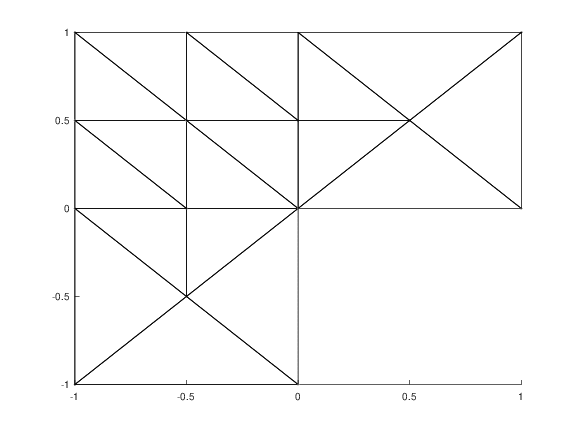
\includegraphics[width =8.5cm]{eta0.9mode5_2}
			&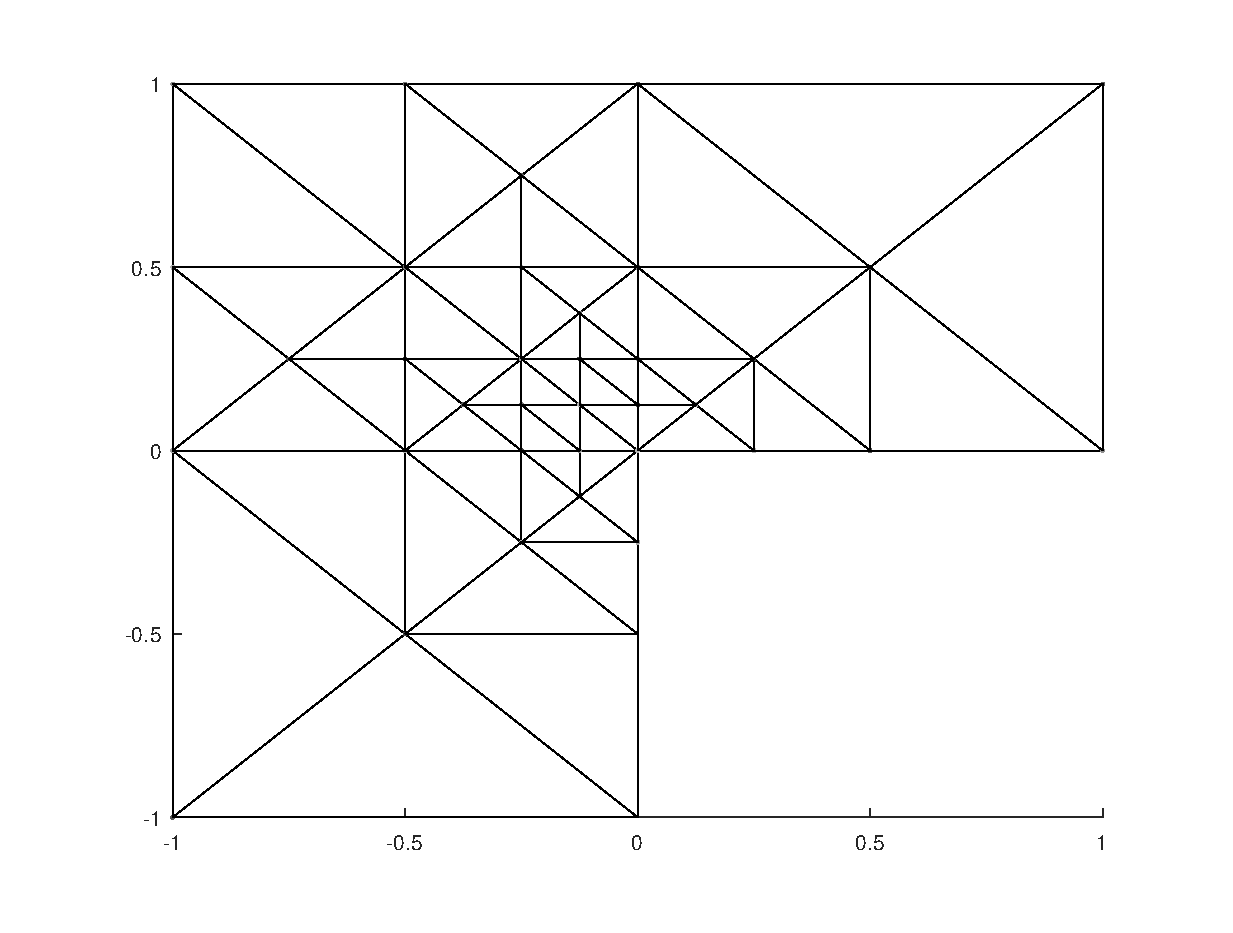
\includegraphics[width =8.5cm]{eta0.9mode5_4}\\
			{\rm (i)}$N$=5  & {\rm (ii)} $N$=23
		\end{tabular}
	\end{center}
	\begin{center}
		\begin{tabular}{c c}
			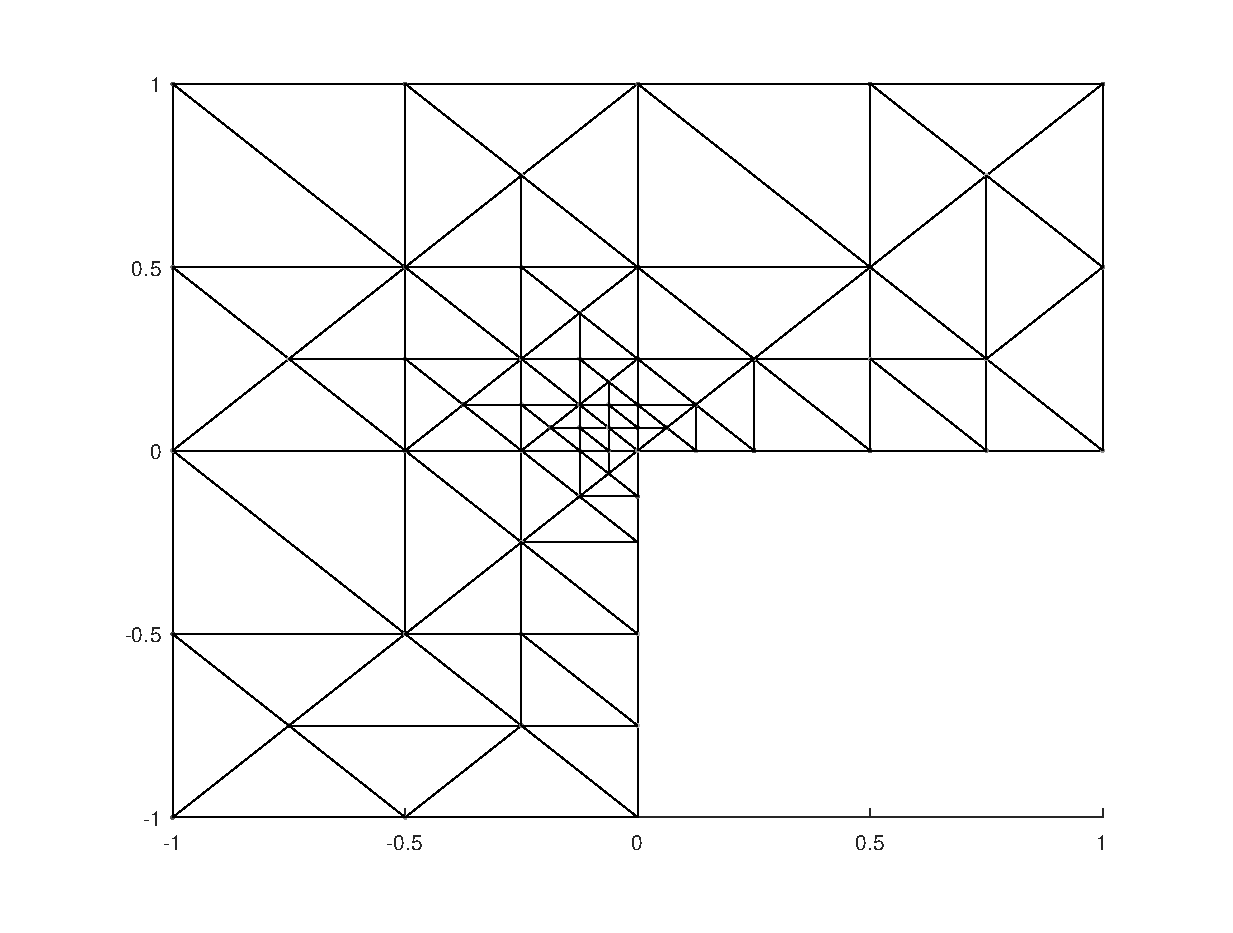
\includegraphics[width =8.5cm]{eta0.9mode5_6}
			&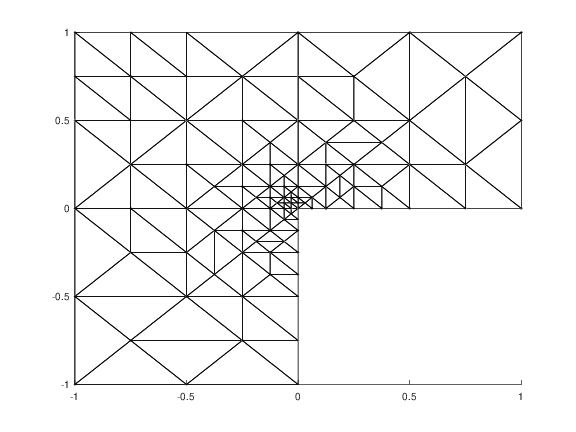
\includegraphics[width =8.5cm]{eta0.9mode5_8} \\
			{\rm (i)} $N$=57 & {\rm (ii)} $N$=79
		\end{tabular}
		\caption{Secuencia de refinamiento adaptativo}
	\end{center}
\end{table}

En las secuencias anteriores podemos notar la selecci\'on de los elementos a refinar donde $\eta_{R,T}>\xi\cdot \eta_{max}$, de {\rm (i)}  a {\rm (ii)} se pasa de 18 a 58 elementos, de {\rm (ii)}  a {\rm (iii)}  se pasa de 58 a 96 elementos y de {\rm (iii)}  a {\rm (iv)} se pasa de 96 a 166 elementos acerc\'andose cada vez mas a la singularidad de la funci\'on $u(r,\theta)$.



\part{Matem\'aticas}

\chapter{Ecuaciones diferenciales}
En est\'e cap\'itulo vamos a entender que es una ecuaci\'on diferencial. 

Para comenzar a formular lo que es una ecuaci\'on diferencial, comencemos explorando lo que es la en s\'i, la palabra ecuaci\'on, de donde proviene, ?`C\'omo hemos trascendido los seres humanos en el pensamiento de las ecuaciones? ?`Para que sirven las ecuaciones y por ende donde aplicarlas? Es un tarea muy dura, pero lo vamos a lograr, formulando  preguntas para ir llegando a respuestas y de estas respuestas dar el salto a lo que yo llamo familiarizaci\'on intelectual. 

?`Por qu\'e planteamos ecuaciones? tratemos de acercarnos a esta pregunta observando la siguiente ecuaci\'on
\begin{equation}\label{equ1.1}
	y+5 = 0
\end{equation}

?`Qu\'e elementos involucrados conocemos en la ecuaci\'on \ref{equ1.1}?

Los n\'umeros 5 y 0, son dos enteros y la variable $y$ representando lo desconocido en la ecuaci\'on, es decir, lo que queremos encontrar, si nos enfocamos en ese sentido, llegaremos a que $y=-5$. 
\begin{equation}
	y(x)=y^{\prime}(x)
\end{equation}
Note que tenemos una igualdad de funciones, una ecuaci\'on que se cumple solo para las funciones que son soluciones de la misma. ?`Cuales son estas funciones? las funciones $c\exp(x)$, de esta manera podemos definir este tipo de ecuaciones, ?`Por qu\'e es importante las ecuaciones diferenciales? ?`Qu\'e fen\'omenos describe el c\'alculo? en intervengan, la distancia, velocidades y aceleraciones.

\begin{definicion}[Ecuaci\'on diferencial]
Una ecuaci\'on diferencial es cualquier ecuaci\'on que contiene las derivadas de una o m\'as variables dependientes con respecto a una o m\'as variables independientes.
\end{definicion}
\begin{ejemplo}
	\begin{align}
		\frac{dy}{dx} + \frac{dz}{dx} &= 2y + z, \\
		\frac{\partial^{2}u}{\partial{x^{2}}} &= \frac{\partial^{2}u}{\partial t^{2}} - 2\frac{\partial u}{\partial t} 
	\end{align}
\end{ejemplo}


\part{Ingles}

\chapter{Frases en ingl\'es}

\begin{description}
	\item[After you: ] Despu\'es de usted.
	\item[Check it out: ] \'Echale un vistazo.
	\item[I guess so: ] Supongo que si.
	\item[What a mess: ] Qu\'e desastre.
	\item[Good for you: ] Bien por ti.			
	
	to get one is hopes up 
\end{description}

\chapter{ Unknown words }
\begin{description}
	\item[Which: ]  cual ; pronombre: que.
	\item[Shall: ]  debera.
	\item [use:  ]  usar.
	\item[brief: ]  breve.
	\item[either:]	conjuci\'on : o, adjetive: Cualquiera de los dos, uno u otro; Adverbio: tambi\'en.
	\item[Roughly speaking: ] mas o menos
	\item[behave: ] comportarse
	\item[obey: ] obedecer
	\item[listed: ] listado
	\item[in that: ] en eso
	\item[for most:] para la mayor\'ia
	\item[may :] poder, ser posible.
	\item[well :] bien
	\item[ to allow for this :] para permitir esto
	\item[rather than  :] m\'as bien que
	\item[itself :] s\'i mismo
	\item[this means :] esto significa
	\item[so are :] tambi\'en lo son
	\item[such :] tal
	\item[below :] abajo
	\item[performance :] actuaci\'on, el rendimiento, desempe\~no
	\item[us out of :]	nosotros fuera de							
	\item[given :]	dado								
	\item[on this	 :]	en este							
	\item[unless :] a no ser que			
	\item[must  :] deber
	\item[we leave it :] lo dejamos
	\item[want  :] desear
	\item[dwell :] residir
	\item[happen :] suceder
	\item[least :] el menos
	\item[Often :] Con frecuencia
	\item[exposure :] exposici\'on
	\item[better :] mejor
	\item[worry :] preocuparse
	\item[about :] sobre						
	\item[vowels :] 
	\item[consonants :]

\end{description}

\chapter{Ingl\'es A1}

Marco Com\'un Europeo de Referencia para las Lenguas (MCER): 

\section{An\'alisis de habilidades}

A continuaci\'on, encontramos un an\'alisis de los diferentes componentes del idioma y las habilidades individuales que un estudiante deber\'ia tener para recibir un certificado A1 de ingles: 

{\bf Compresi\'on auditiva}

Los estudiantes de nivel A1 deberi\'an ser capaces de entender un ingl\'es est\'andar simple, siempre y cuando sea hablado con claridad por alguien paciente y dispuesto ayudar. Especificamente, deberi\'an poder reconocer frases y palabras comunes, relacionadas con ellos mismos, su entorno y aquellos cercanos a ellos. Adem\'as, deber\'ian entender cosas como los n\'umeros, direcciones y otras instrucciones muy b\'asicas en ingl\'es.

Welcome everyone to the basic English course. A one for beginners. I'm your teacher, kira Sage, nice to meet you. Who am i? I am from the U.S.A I have taught C level executives and software engineers at companies like google skhynix, Tesla, Sony and more. I have nine years of teaching experience in countries like Usa and Japan. Here are a couple of interesting facts about me. I have visited four of the six Disneyland's around the world. This is me at Star Wars, Galaxy edge in Anaheim California. Also i have Master's degree in teaching T. Saw that means I can teach teachers and learners like you in this course you will learn the alphabet ah and un sentences with it's plural forms, sentences with there are numbers, colors, subject pronouns, professions, greetings, negative and interrogative statements, possessive adjectives. Days of the week, your hobbies, questions with what's your and to review everything from this course we'll have to wrap up class. Here's you'll learn all of the course concepts through worksheets, find the worsheets in the resources section through interactive quizzes and through interactive explanations on an imaginary website called plattso plattso is where we practice english so we can make friends online. Are you ready for this  fun adventure? I'll see you in the next class.


Bienvenido todos al curso the Ingles b\'asico. A1 para comenzar 



\begin{verbatim}
Intento 1: 
Welcome everyone to the Black Sea English course A1 for beginners I
 am here t-shirt carousel nice to me you Hoang I who on my I'm from
 the USA I have to see level executive a software engineer and companies
 like Google sky and Tesla Sony and more I cannae jeers of teaching experience in countries like USA and Japan he are Kobe of interesting
 facts about me I had visits of the seeds Disneyland around the world this is me at Star Wars Galaxy Edge in Anaheim California also I have
 massive degree in teaching t so that means can teach t-shirts in Learners like you in this course you will learn the alphabet I'm on
 sentence with it's pure Air Force sentence with there are numbers caller surgeon pronounce profession where teens interrogative
 status. Osiria Jetties days of the weave your hobbies question with what you ain't to review everything from this course we wait
 we all have to grab a glass of the course Concepts world war ships find a wall sheets in the results section throw in charity
 crisis and throw into righteous play Nations oh imagine a website called black English so we can make friends only are you
 ready for this funeral bencher Adventure I also see you in the next class.
         
         
 Segundo intento: 
 welcome everyone to the basic English course. a wife for beginners at
  Food dock. Avon for beginners sorry please thought a blunt for 
  beginners. A1 for beginners. I am your teacher call Ma Kira say Asahi 
  call Mama, nice to meet you. who I who am I. I am from the USA. I 
  hopped out I have towels. IHOP takeout see Liberty Security in Sulphur 
  and genius and companies like Google Skynet call mistakes Le gamma 
  Sony a moor Anne Moore Anne Moore Sony and more. I have 9 years of 
  teaching experience in countries like USA in Japan. Cher here. T R A 
  Copley. here are a couple off interesting facts about me. I had visit 
  visit. I had visited full of the sea Disneyland around the world. this 
  is me and it's sad worse, Galaxy Edge in Anaheim California. also I 
  have. also I had Mercer metzer Meister Meister mustard master. also I 
  heart muscle is degree and teach t. all soup IHOP Massillon he's they 
  greet and teach tea. soda means I can teach t-shirts in layers
\end{verbatim} 

\url{https://www.youtube.com/watch?v=EVNhOAEW784}

\url{https://howjsay.com/how-to-pronounce-taught}
Para pronuciar Taught comience colocando su lengua detr\'as de sus dientes superiores y agregue el sonidoo AH corto y abierto termine con una T colocando su lengua detr\'as de sus dientes superiores



Numbers class Two: 

Welcome to the 1st Module. This english fundamentals in this module.
In this Module you will learn the 
\begin{enumerate}
	\item alphabet.
	\item A and N 
	\item sentences with it's plural forms
	\item  and sentences with there are
\end{enumerate}
 this is the alphabet. Now let's go and learn on platzo.
 
 Welcome to plattzo. Now loading oh do you know what this is?
 
 it's capture. We need letters to unlock the capture. Well let's learn in this class. 
 
 You will learn the letters of the english alphabet. In the English Alphabet there are 26 letters. Let's practice. I will say a letter an repeat after me. Ready, let's go. A B Bravo. C D E. Excellent F G. Googd job H I J K, keep it up. L M magnificent N. Nice work. O P perfect Q R S super T terrific. U V very goog W wonderful X. Why Z in some countries this letter is zed.
 
 Now, you know the letters of the alphabet? A B C D E F G H I J K L M N O P Q R S T u v w x, y z. OR ZED. 	Let's use these letters to unlock the capture on plattzo.
 
 The capture says a phrase, not a robot. Let's spell the phrase letter by letter N O T A R O B O T. You did it. You unlock the capture. 
 
 Great job. it's your turn. Here is the alphabet but some letters are missing. 
 
 Type, the missing letters in the discussion panel. 
 Don't forget to download your worksheet from the resources section that worksheet is your plattzo profile. Complete the user name area of your plattzo profile on your woorksheet, keep this worksheet with you at all times. We will complete your plattzo profile in each module of this course. So keep ir ready for extra practice. Type your user name in the discussion panel.
 
 My user name is Kira K I R A. I'll see you in the next class.
 
 
 Email: jcausilmartinez@gmail.com
 
 Number phone: 314 796 81 19.
 
 User name: Javier Andres Causil Martínez


My introducction in is Spanish:  

Hola mi nombre es Javier Andr\'es Causil Mart\'inez, soy de Colombia del departamento de Antioquia en la ciudad de Caucasia. Tengo 27 a\~nos, soy Matem\'atico  de la Universidad de Antioquia y programador, me gusta la m\'usica, hacer deporte, aprender cosas nuevas. Siento gran pasi\'on por la m\'usica cl\'asica. 



\subsection{A and AN}

A and AN refer to only one person, place, or thing, or noun.

An is an article that we use with vowels. Vowels are ``a'', ``e'', ``i'', ``o'', ``u''

Use ``an'' with these vowels. Now, let's them together on Platzo.

``A'' is the article we use with consonants.

Be careful! there is an exception. The most common exception is with the letter U.

Now you can use ``a'' and ``an'' with vowels and consonants.

\subsection{IT'S SENTENCES}

In this class, you will learn sentences with ``it's''.

First, use ``it's'' or ``'it is' with a noun, 

it is + a person: a thing: an item: a place

We can make sentences with ``it's, an article, and a noun''.

In this class, you wil learn forms plurals, 

\subsection{Plural forms}

The most common plural form is to add ``s'' at the end of the word. Para otras palabras que terminan con ``S,SH,CH,X'' y ``Z'', we add ``es'' to the end of those words.

Words with ``y'' are special. because when a ``y'' is next to a vowel, we just add ``S'', when a ``y'' is next to a consonant, we change the ``y'' to ``i'' and add ``es''.

\part{Lecturas de libros}

\section{Ultralearning}

Comienza con la ilusi\'on de estudiar en el MIT, pero t\'ermina estudiando negocios en la Universidad de Manitoba, una escuela Canadiense de rango medio, ya que era la que pod\'ia pagar. Pero al terminar la carrera concluyo que se equivoco de carrera cuatro a\~nos mas tarde se da cuenta de una especializaci\'on en administraci\'on y de inform\'atica 

\subsection{Why Ultralearning Matters}

Cu\'ando aplicar el ultraaprendizaje 

\begin{enumerate}
	\item es seguir ultralearning a tiempo parcial.
	\item es buscar el ultraaprendizaje durante las brechas en el trabajo y la escuela.
	\item Es integrar los principios del ultraaprendizaje en el tiempo y la energía que ya dedica al aprendizaje.
	
\end{enumerate}


\subsection{El valor del ultraaprendizaje}

La capacidad de adquirir habilidades duras de manera efectiva y eficiente es inmensamente valiosa. No solo eso, sino que las tendencias actuales en econom\'ia, educaci\'on y tecnolog\'ia van a exacerbar la diferencia entre quienes tienen esta habilidad y quienes no la tienen.

\subsection{Como convertirse en un ultraaprendiz}

Primeros pasos de un ultraaprendiz novato


Principios para convertirse en ultraaprendiz


\begin{verbatim}
1. METALEARNING: PRIMERO DIBUJAR UN MAPA. Comience por aprender cómo aprender el tema o la habilidad que desea abordar. Descubra cómo hacer una buena investigación y cómo aprovechar sus competencias pasadas para aprender nuevas habilidades más fácilmente.

2. ENFOQUE: AFILA TU CUCHILLO. Cultivar la capacidad de concentración. Dedique períodos de tiempo en los que pueda concentrarse en el aprendizaje y haga que sea fácil hacerlo.

3. SERIEDAD: VAYA DERECHO. Aprende haciendo aquello en lo que quieres ser bueno. No lo cambie por otras tareas, solo porque son más convenientes o cómodas.

4. EJERCICIO: ATACA TU PUNTO MÁS DÉBIL. Sea implacable en la mejora de sus puntos más débiles. Divida las habilidades complejas en partes pequeñas; luego domine esas partes y vuelva a construirlas juntas.

5. RECUPERACIÓN: PRUEBA PARA APRENDER. Las pruebas no son simplemente una forma de evaluar el conocimiento, sino una forma de crearlo. Ponte a prueba antes de sentirte seguro y oblígate a recordar activamente la información en lugar de revisarla pasivamente.

6.COMENTARIOS: NO EVITE LOS GOLPES. La retroalimentación es dura e incómoda. Sepa cómo usarlo sin dejar que su ego se interponga en el camino. Extraiga la señal del ruido, para que sepa a qué prestar atención y qué ignorar.

7. RETENCIÓN: NO LLENE UN CUBO CON FUGAS. Entiende lo que olvidas y por qué. Aprende a recordar las cosas no solo por ahora sino para siempre.

8. INTUICIÓN: PROFUNDICE ANTES DE CONSTRUIR. Desarrolla tu intuición a través del juego y la exploración de conceptos y habilidades. Entiende cómo funciona el entendimiento, y no recurras a trucos baratos de memorización para evitar saber las cosas en profundidad.

9. EXPERIMENTACIÓN: EXPLORA FUERA DE TU ZONA DE CONFORT. Todos estos principios son solo puntos de partida. El verdadero dominio proviene no solo de seguir el camino recorrido por otros, sino de explorar posibilidades que aún no han imaginado.
\end{verbatim}

\section{Principio 1}

\subsection{What Is Metalearning?}

Aprehender sobre el aprendizaje

El poder de su mapa de metaaprendizaje

Ser capaz de ver c\'omo funciona un tema, qu\'e tipo de habilidades e informaci\'on se deben dominar y qu\'e m\'etodos est\'an disponibles para hacerlo de manera m\'as efectiva es la base del \'exito de todos los proyectos de ultraaprendizaje.

\begin{verbatim}
Una vez que haya entendido por qué está aprendiendo, puede comenzar a ver cómo se estructura el conocimiento en su materia. Una buena manera de hacer esto es escribir en una hoja de papel tres columnas con los títulos “Conceptos”, “Hechos” y “Procedimientos”. Luego haga una lluvia de ideas sobre todas las cosas que necesitará aprender. No importa si la lista está perfectamente completa o precisa en esta etapa. Siempre puedes revisarlo más tarde. Su objetivo aquí es obtener un primer pase difícil. Una vez que comience a aprender, puede ajustar la lista si descubre que sus categorías no son del todo correctas.
\end{verbatim}

Primera columna de conceptos  si algo necesita ser entendido, no solo memorizado, lo pongo en esta columna en lugar de la segunda columna de hechos.
\begin{verbatim}
	1. METALEARNING: PRIMERO DIBUJAR UN MAPA. Comience por aprender cómo aprender el tema o la habilidad que desea abordar. Descubra cómo hacer una buena investigación y cómo aprovechar sus competencias pasadas para aprender nuevas habilidades más fácilmente.
	
	2. ENFOQUE: AFILA TU CUCHILLO. Cultivar la capacidad de concentración. Dedique períodos de tiempo en los que pueda concentrarse en el aprendizaje y haga que sea fácil hacerlo. 
	
	3. SERIEDAD: VAYA DERECHO. Aprende haciendo aquello en lo que quieres ser bueno. No lo cambie por otras tareas, solo porque son más convenientes o cómodas.
	
	4. EJERCICIO: ATACA TU PUNTO MÁS DÉBIL. Sea implacable en la mejora de sus puntos más débiles. Divida las habilidades complejas en partes pequeñas; luego domine esas partes y vuelva a construirlas juntas.
	
	5. RECUPERACIÓN: PRUEBA PARA APRENDER. Las pruebas no son simplemente una forma de evaluar el conocimiento, sino una forma de crearlo. Ponte a prueba antes de sentirte seguro y oblígate a recordar activamente la información en lugar de revisarla pasivamente. 
	
	6.COMENTARIOS: NO EVITE LOS GOLPES. La retroalimentación es dura e incómoda. Sepa cómo usarlo sin dejar que su ego se interponga en el camino. Extraiga la señal del ruido, para que sepa a qué prestar atención y qué ignorar.
	
	7. RETENCIÓN: NO LLENE UN CUBO CON FUGAS. Entiende lo que olvidas y por qué. Aprende a recordar las cosas no solo por ahora sino para siempre. 
	
	8. INTUICIÓN: PROFUNDICE ANTES DE CONSTRUIR. Desarrolla tu intuición a través del juego y la exploración de conceptos y habilidades. Entiende cómo funciona el entendimiento, y no recurras a trucos baratos de memorización para evitar saber las cosas en profundidad. 
	
	9. EXPERIMENTACIÓN: EXPLORA FUERA DE TU ZONA DE CONFORT. Todos estos principios son solo puntos de partida. El verdadero dominio proviene no solo de seguir el camino recorrido por otros, sino de explorar posibilidades que aún no han imaginado. 
\end{verbatim}

\section{Principio 1}

\subsection{What Is Metalearning?}

Aprehender sobre el aprendizaje

El poder de su mapa de metaaprendizaje

Ser capaz de ver c\'omo funciona un tema, qu\'e tipo de habilidades e informaci\'on se deben dominar y qu\'e m\'etodos est\'an disponibles para hacerlo de manera m\'as efectiva es la base del \'exito de todos los proyectos de ultraaprendizaje.

\begin{verbatim}
	Una vez que haya entendido por qué está aprendiendo, puede comenzar a ver cómo se estructura el conocimiento en su materia. Una buena manera de hacer esto es escribir en una hoja de papel tres columnas con los títulos “Conceptos”, “Hechos” y “Procedimientos”. Luego haga una lluvia de ideas sobre todas las cosas que necesitará aprender. No importa si la lista está perfectamente completa o precisa en esta etapa. Siempre puedes revisarlo más tarde. Su objetivo aquí es obtener un primer pase difícil. Una vez que comience a aprender, puede ajustar la lista si descubre que sus categorías no son del todo correctas.
	
	Primera columna de conceptos  si algo necesita ser entendido, no solo memorizado, lo pongo en esta columna en lugar de la segunda columna de hechos.
	
	En la segunda columna, escribe todo lo que necesites memorizar. Los hechos son cualquier cosa que sea suficiente si puedes recordarlos. No es necesario que los entienda demasiado profundamente, siempre y cuando pueda recordarlos en las situaciones adecuadas. 
	
	En la tercera columna, escribe todo lo que necesites practicar. Los procedimientos son acciones que deben realizarse y es posible que no impliquen mucho pensamiento consciente.
	
	Una vez que haya terminado su lluvia de ideas, subraye los conceptos, hechos y procedimientos que serán más desafiantes. Esto le dará una buena idea de cuáles serán los principales cuellos de botella de aprendizaje y puede comenzar a buscar métodos y recursos para superar esas dificultades.
	
	Ahora que ha respondido dos preguntas, por qué está aprendiendo y qué está aprendiendo, es hora de responder la pregunta final: ¿Cómo va a aprenderlo? Sugiero seguir dos métodos para responder cómo aprenderá algo: Benchmarking y el Método de énfasis/exclusión. (Benchmarking and the Emphasize/Exclude Method.)
	
	Las luchas con el enfoque que tienen las personas generalmente vienen en tres variedades amplias: comenzar, mantener y optimizar la calidad del enfoque de uno. Los ultraalumnos son implacables a la hora de encontrar soluciones para manejar estos tres problemas, que forman la base de la capacidad de concentrarse bien y aprender profundamente.
	
	 Examinemos algunas de las tácticas que usan los ultraestudiantes para maximizar este principio y aprovechar las deficiencias de la educación más típica. 
	 
	 Táctica 1: aprendizaje basado en proyectos Muchos ultraestudiantes optan por proyectos en lugar de clases para aprender las habilidades que necesitan.
	 
	 Táctica 2: Aprendizaje inmersivo
	 
	 La inmersión es el proceso de rodearse del entorno objetivo en el que se practica la habilidad. Esto tiene la ventaja de requerir una cantidad de práctica mucho mayor de lo que sería típico, además de exponerlo a una gama más completa de situaciones en las que se aplica la habilidad.
	 
	 Táctica 3: El método del simulador de vuelo
	 
	 Es simular el entorno, aproximarse al entorno real a través de uno muy parecido.
	 
	 Táctica 4: El enfoque exagerado
	 
	 El último método que encontré para mejorar la franqueza es aumentar el desafío, de modo que el nivel de habilidad requerido esté completamente contenido dentro de la meta establecida. 
	 
	 Aprenda directamente de la fuente
	 
	 El aprendizaje directo es uno de los sellos distintivos de muchos de los proyectos exitosos de ultraaprendizaje que he encontrado, particularmente por lo diferente que puede ser del estilo de educación al que la mayoría de nosotros estamos acostumbrados.
	 
	 Los ultraestudiantes, por el contrario, emplean con frecuencia lo que llamaré el enfoque Direct-Then-Drill.
	 
	 El primer paso es tratar de practicar la habilidad directamente. Esto significa averiguar dónde y cómo se usará la habilidad y luego tratar de igualar esa situación lo más cerca posible al practicar. 
	 
	  El siguiente paso es analizar la habilidad directa y tratar de aislar los componentes que son pasos determinantes en su rendimiento o subhabilidades que encuentra difíciles de mejorar porque hay demasiadas otras cosas sucediendo para que usted se concentre en ellas.
	  
	  El paso final es volver a la práctica directa e integrar lo que has aprendido. Esto tiene dos propósitos. La primera es que, incluso en ejercicios bien diseñados, habrá problemas de transferencia debido al hecho de que lo que antes era una habilidad aislada debe trasladarse a un contexto nuevo y más complejo. Piense en esto como si estuviera construyendo el tejido conectivo para unir los músculos que fortaleció por separado. La segunda función de este paso es verificar si su ejercicio fue bien diseñado y apropiado. Muchos intentos de aislar un ejercicio pueden terminar en fracaso porque el ejercicio realmente no llega al corazón de lo que era difícil en la práctica real. 
	  
	  Tácticas para diñar simulacros: 
	  
	  
	 
\end{verbatim}



%\addcontentsline{toc}{chapter}{\numberline{}Bibliograf�a}
\end{document}